\documentclass[]{article}
\usepackage{lmodern}
\usepackage{amssymb,amsmath}
\usepackage{ifxetex,ifluatex}
\usepackage{fixltx2e} % provides \textsubscript
\ifnum 0\ifxetex 1\fi\ifluatex 1\fi=0 % if pdftex
  \usepackage[T1]{fontenc}
  \usepackage[utf8]{inputenc}
\else % if luatex or xelatex
  \ifxetex
    \usepackage{mathspec}
  \else
    \usepackage{fontspec}
  \fi
  \defaultfontfeatures{Ligatures=TeX,Scale=MatchLowercase}
\fi
% use upquote if available, for straight quotes in verbatim environments
\IfFileExists{upquote.sty}{\usepackage{upquote}}{}
% use microtype if available
\IfFileExists{microtype.sty}{%
\usepackage{microtype}
\UseMicrotypeSet[protrusion]{basicmath} % disable protrusion for tt fonts
}{}
\usepackage[margin=1in]{geometry}
\usepackage{hyperref}
\hypersetup{unicode=true,
            pdftitle={TMA4268 Statistical Learning V2019},
            pdfauthor={Mette Langaas and Thea Roksvåg, Department of Mathematical Sciences, NTNU},
            pdfborder={0 0 0},
            breaklinks=true}
\urlstyle{same}  % don't use monospace font for urls
\usepackage{color}
\usepackage{fancyvrb}
\newcommand{\VerbBar}{|}
\newcommand{\VERB}{\Verb[commandchars=\\\{\}]}
\DefineVerbatimEnvironment{Highlighting}{Verbatim}{commandchars=\\\{\}}
% Add ',fontsize=\small' for more characters per line
\usepackage{framed}
\definecolor{shadecolor}{RGB}{248,248,248}
\newenvironment{Shaded}{\begin{snugshade}}{\end{snugshade}}
\newcommand{\AlertTok}[1]{\textcolor[rgb]{0.94,0.16,0.16}{#1}}
\newcommand{\AnnotationTok}[1]{\textcolor[rgb]{0.56,0.35,0.01}{\textbf{\textit{#1}}}}
\newcommand{\AttributeTok}[1]{\textcolor[rgb]{0.77,0.63,0.00}{#1}}
\newcommand{\BaseNTok}[1]{\textcolor[rgb]{0.00,0.00,0.81}{#1}}
\newcommand{\BuiltInTok}[1]{#1}
\newcommand{\CharTok}[1]{\textcolor[rgb]{0.31,0.60,0.02}{#1}}
\newcommand{\CommentTok}[1]{\textcolor[rgb]{0.56,0.35,0.01}{\textit{#1}}}
\newcommand{\CommentVarTok}[1]{\textcolor[rgb]{0.56,0.35,0.01}{\textbf{\textit{#1}}}}
\newcommand{\ConstantTok}[1]{\textcolor[rgb]{0.00,0.00,0.00}{#1}}
\newcommand{\ControlFlowTok}[1]{\textcolor[rgb]{0.13,0.29,0.53}{\textbf{#1}}}
\newcommand{\DataTypeTok}[1]{\textcolor[rgb]{0.13,0.29,0.53}{#1}}
\newcommand{\DecValTok}[1]{\textcolor[rgb]{0.00,0.00,0.81}{#1}}
\newcommand{\DocumentationTok}[1]{\textcolor[rgb]{0.56,0.35,0.01}{\textbf{\textit{#1}}}}
\newcommand{\ErrorTok}[1]{\textcolor[rgb]{0.64,0.00,0.00}{\textbf{#1}}}
\newcommand{\ExtensionTok}[1]{#1}
\newcommand{\FloatTok}[1]{\textcolor[rgb]{0.00,0.00,0.81}{#1}}
\newcommand{\FunctionTok}[1]{\textcolor[rgb]{0.00,0.00,0.00}{#1}}
\newcommand{\ImportTok}[1]{#1}
\newcommand{\InformationTok}[1]{\textcolor[rgb]{0.56,0.35,0.01}{\textbf{\textit{#1}}}}
\newcommand{\KeywordTok}[1]{\textcolor[rgb]{0.13,0.29,0.53}{\textbf{#1}}}
\newcommand{\NormalTok}[1]{#1}
\newcommand{\OperatorTok}[1]{\textcolor[rgb]{0.81,0.36,0.00}{\textbf{#1}}}
\newcommand{\OtherTok}[1]{\textcolor[rgb]{0.56,0.35,0.01}{#1}}
\newcommand{\PreprocessorTok}[1]{\textcolor[rgb]{0.56,0.35,0.01}{\textit{#1}}}
\newcommand{\RegionMarkerTok}[1]{#1}
\newcommand{\SpecialCharTok}[1]{\textcolor[rgb]{0.00,0.00,0.00}{#1}}
\newcommand{\SpecialStringTok}[1]{\textcolor[rgb]{0.31,0.60,0.02}{#1}}
\newcommand{\StringTok}[1]{\textcolor[rgb]{0.31,0.60,0.02}{#1}}
\newcommand{\VariableTok}[1]{\textcolor[rgb]{0.00,0.00,0.00}{#1}}
\newcommand{\VerbatimStringTok}[1]{\textcolor[rgb]{0.31,0.60,0.02}{#1}}
\newcommand{\WarningTok}[1]{\textcolor[rgb]{0.56,0.35,0.01}{\textbf{\textit{#1}}}}
\usepackage{graphicx,grffile}
\makeatletter
\def\maxwidth{\ifdim\Gin@nat@width>\linewidth\linewidth\else\Gin@nat@width\fi}
\def\maxheight{\ifdim\Gin@nat@height>\textheight\textheight\else\Gin@nat@height\fi}
\makeatother
% Scale images if necessary, so that they will not overflow the page
% margins by default, and it is still possible to overwrite the defaults
% using explicit options in \includegraphics[width, height, ...]{}
\setkeys{Gin}{width=\maxwidth,height=\maxheight,keepaspectratio}
\IfFileExists{parskip.sty}{%
\usepackage{parskip}
}{% else
\setlength{\parindent}{0pt}
\setlength{\parskip}{6pt plus 2pt minus 1pt}
}
\setlength{\emergencystretch}{3em}  % prevent overfull lines
\providecommand{\tightlist}{%
  \setlength{\itemsep}{0pt}\setlength{\parskip}{0pt}}
\setcounter{secnumdepth}{0}
% Redefines (sub)paragraphs to behave more like sections
\ifx\paragraph\undefined\else
\let\oldparagraph\paragraph
\renewcommand{\paragraph}[1]{\oldparagraph{#1}\mbox{}}
\fi
\ifx\subparagraph\undefined\else
\let\oldsubparagraph\subparagraph
\renewcommand{\subparagraph}[1]{\oldsubparagraph{#1}\mbox{}}
\fi

%%% Use protect on footnotes to avoid problems with footnotes in titles
\let\rmarkdownfootnote\footnote%
\def\footnote{\protect\rmarkdownfootnote}

%%% Change title format to be more compact
\usepackage{titling}

% Create subtitle command for use in maketitle
\providecommand{\subtitle}[1]{
  \posttitle{
    \begin{center}\large#1\end{center}
    }
}

\setlength{\droptitle}{-2em}

  \title{TMA4268 Statistical Learning V2019}
    \pretitle{\vspace{\droptitle}\centering\huge}
  \posttitle{\par}
  \subtitle{Module 9: SUPPORT VECTOR MACHINES}
  \author{Mette Langaas and Thea Roksvåg, Department of Mathematical Sciences,
NTNU}
    \preauthor{\centering\large\emph}
  \postauthor{\par}
      \predate{\centering\large\emph}
  \postdate{\par}
    \date{week 11 2019}

\usepackage{booktabs}
\usepackage{makecell}

\begin{document}
\maketitle

{
\setcounter{tocdepth}{2}
\tableofcontents
}
Last changes: (13.05 typos from student, 09.03: first version)

\#Introduction

This field dates back to the 1990s in computer science, and in this
presentation we put emphasis on the underlying motivation and
connections to linear algebra, optimization theory and statistics.

We will only cover classification, and in particular two-class problems.

\hypertarget{learning-material-for-this-module}{%
\subsection{Learning material for this
module}\label{learning-material-for-this-module}}

\begin{itemize}
\tightlist
\item
  James et al (2013): An Introduction to Statistical Learning. Chapter
  9.\\
\item
  \href{https://www.math.ntnu.no/emner/TMA4268/2019v/notes/M9notes.pdf}{Classnotes
  11.03.2019}
\end{itemize}

Some of the figures in this presentation are taken from (or are inspired
by) ``An Introduction to Statistical Learning, with applications in R''
(Springer, 2013) with permission from the authors: G. James, D. Witten,
T. Hastie and R. Tibshirani.

\begin{center}\rule{0.5\linewidth}{\linethickness}\end{center}

\hypertarget{topics}{%
\subsection{Topics}\label{topics}}

\begin{itemize}
\tightlist
\item
  \protect\hyperlink{intro}{Motivation}
\item
  \protect\hyperlink{mmc}{Maximal margin classifier}
\item
  \protect\hyperlink{svc}{Support vector classifier}
\item
  \protect\hyperlink{svm}{Support vector machines}
\item
  \protect\hyperlink{ext}{Extensions}
\item
  \protect\hyperlink{comp}{Comparisons}
\item
  \protect\hyperlink{summing}{Summing up}
\item
  \protect\hyperlink{recex}{Recommended exercises}
\item
  \protect\hyperlink{Rpackages}{R Packages}
\item
  \protect\hyperlink{further}{References}
\end{itemize}

\begin{center}\rule{0.5\linewidth}{\linethickness}\end{center}

\hypertarget{motivation}{%
\subsection{Motivation}\label{motivation}}

Suppose that you are interested in the distribution of two tree types:
redwood and pines. You have three different study areas in which these
trees grow. Your study areas are visualized in the three figures below
with orange points indicating the position of a redwood tree and green
points indicating the position of a pine tree in a forest.

\begin{center}\rule{0.5\linewidth}{\linethickness}\end{center}

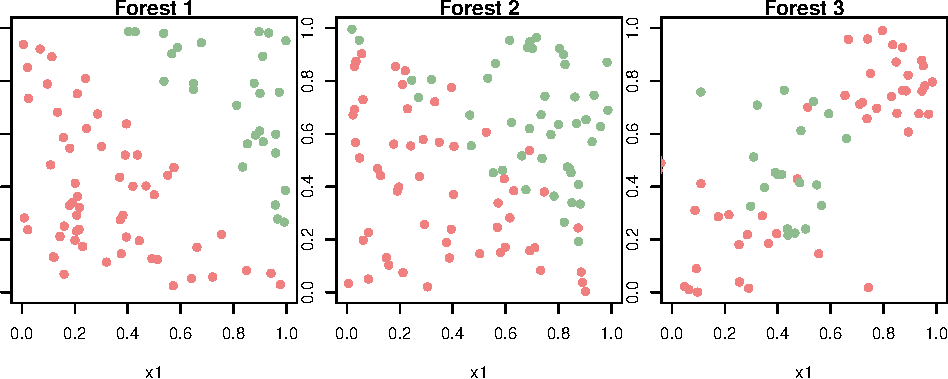
\includegraphics{9SVM_files/figure-latex/unnamed-chunk-1-1.pdf}

Assume you want to build one continuous fence to separate the two tree
types in each of the three study areas. \textbf{Where should you build
the fence?}

\begin{center}\rule{0.5\linewidth}{\linethickness}\end{center}

For Forest 1 the choice seems easy: The orange and green points are
clearly separated and the fence can be built anywhere inside the band
that separates them. However, we can draw infinitely many straight lines
that all separate the two tree types, and we should take into account
that the trees reproduce and that we want future pines and future
redwoods to grow up on the correct side of the fence.

The problem gets more complicated for Forest 2. A linear fence still
seems like a good idea, but in this case the two tree types can not be
perfectly separated. You have to allow some of the trees to be on the
wrong side of the fence. The complexity of the problem is further
increased for Forest 3. It is not possible to separate the two tree
types by a straight line without getting a large number of
misclassifications. Here, a circular fence around the pine trees seems
like a reasonable choice.

\begin{center}\rule{0.5\linewidth}{\linethickness}\end{center}

Forest 1 illustrates the problem of finding an \textbf{optimal
separating hyperplane} for a dataset. In this module you are going to
learn a method for finding optimal hyperplanes called \textbf{Maximal
Margin hyperplanes}.

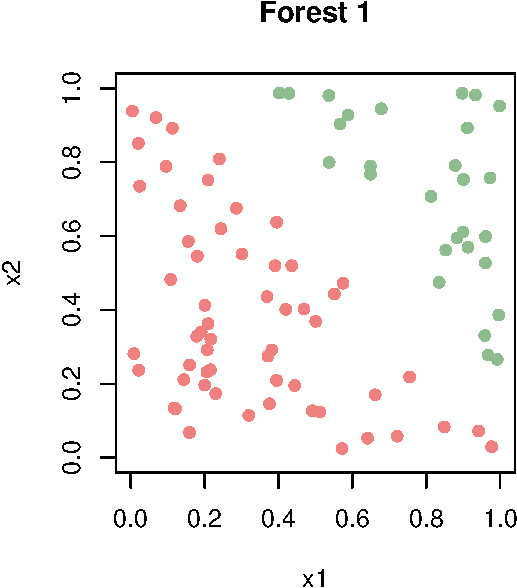
\includegraphics{9SVM_files/figure-latex/unnamed-chunk-2-1.pdf}

\begin{center}\rule{0.5\linewidth}{\linethickness}\end{center}

You are also going to learn how you can find an optimal separating
hyperplane when your data cannot be perfectly separated by a straight
line, as in Forest 2. This leads to a classifier called a
\textbf{Support Vector Classifier} or a \textbf{Soft Margin Classifier}.

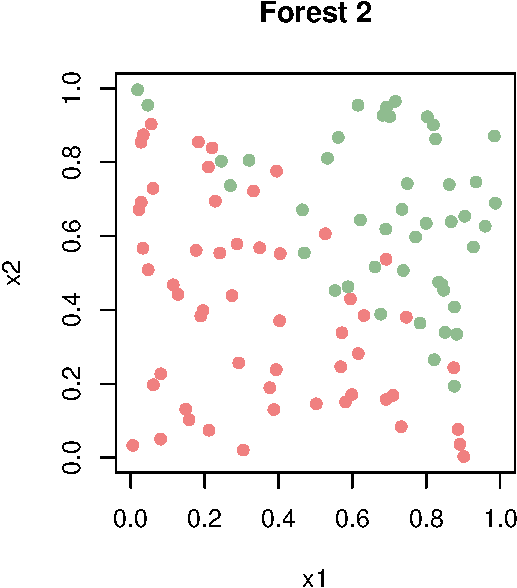
\includegraphics{9SVM_files/figure-latex/unnamed-chunk-3-1.pdf}

\begin{center}\rule{0.5\linewidth}{\linethickness}\end{center}

The Support vector classifier can be generalised to an approach that
produces non-linear decision boundaries. This is called the
\textbf{Support Vector Machine} (SVM) and is useful when the data is
distributed as illustrated in Forest 3.

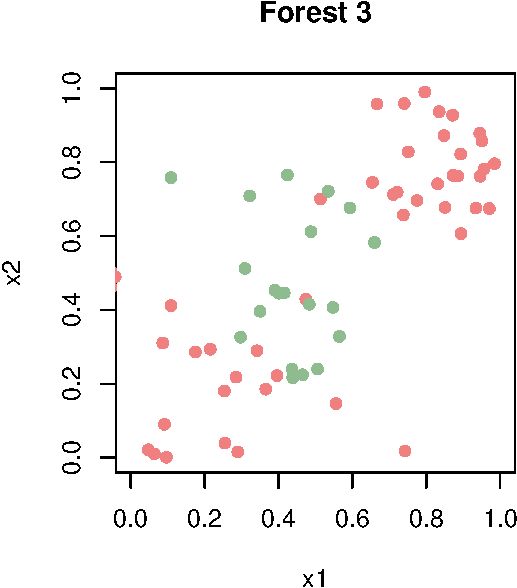
\includegraphics{9SVM_files/figure-latex/unnamed-chunk-4-1.pdf}

\begin{center}\rule{0.5\linewidth}{\linethickness}\end{center}

The reason why we want to separate the data by finding an optimal
hyperplane or a separating cruve, is that we want to use it for
classification. In our example: Is it likely that a random seed found at
location \((0.8,0.4)\) becomes a redwood or a pine tree given the
observed data? We classify a new observation based on which side of the
decision boundary it falls into.

The methods presented in this module are intended for binary
classification, i.e \textbf{classification with two classes}, but
extensions to more than two classes are briefly mentioned.

\begin{center}\rule{0.5\linewidth}{\linethickness}\end{center}

\hypertarget{dataset}{%
\subsection{Dataset}\label{dataset}}

The three forests will be used as illustrative examples throughout the
module. In this dataset we have two covariates,

\emph{the \(x_1\)- and the \(x_2\)-coordinate of each tree in the
forest, and } the response is the tree type, either \(pine\) or
\(redwood\).

The class \(pine\) is stored as 1 in our dataset, while \(redwood\) is
stored as -1. (Yes, we have used 0 and 1 before.)

\begin{center}\rule{0.5\linewidth}{\linethickness}\end{center}

Our goal is to make a classifier for random seeds that we find on the
ground for each of the three forests. The locations of the seeds are
shown in the figure below (black circles), and we want to classify the
seeds as either pine seeds or redwood seeds given our observations.
Thus, the point patterns above can be thought of as the training set,
while the point pattern generated by the black circles can be thought of
as the test set.

\begin{center}\rule{0.5\linewidth}{\linethickness}\end{center}

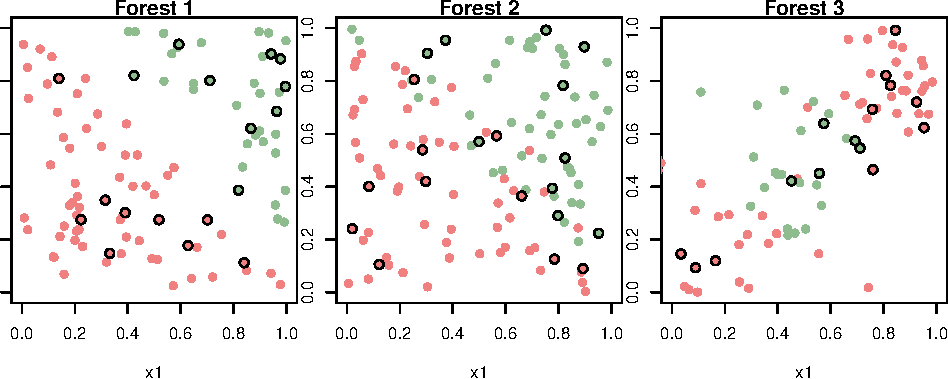
\includegraphics{9SVM_files/figure-latex/unnamed-chunk-5-1.pdf}

\begin{center}\rule{0.5\linewidth}{\linethickness}\end{center}

\hypertarget{maximal-margin-classifier}{%
\section{Maximal Margin Classifier}\label{maximal-margin-classifier}}

\hypertarget{hyperplane}{%
\subsection{Hyperplane}\label{hyperplane}}

A \textbf{hyperplane} in p-dimensions is defined as

\[\beta_0+\beta_1 X_1 + \beta_2 X_2 +...+\beta_p X_p=\beta_0+{\bf x}^T {\boldsymbol \beta}=0.\]
and is a \(p-1\) dimensional subspace.

\begin{itemize}
\tightlist
\item
  If a point \(X=(X_1,X_2,...,X_p)^T\) satisfies the above equation, it
  lies on the hyperplane.
\item
  If \(\beta_0=0\) the hyperplane goes through the origin (origo).
\item
  The vector \(\beta_1, \ldots, \beta_p\) (not including \(\beta_0\)) is
  called the normal vector and points in the direction orthogonal to the
  hyperplane.
\end{itemize}

\begin{center}\rule{0.5\linewidth}{\linethickness}\end{center}

If a point \(X=(X_1,X_2,...,X_p)^T\) satisfies

\begin{itemize}
\tightlist
\item
  \(\beta_0+\beta_1 X_1 + \beta_2 X_2 +...+\beta_p X_p=\beta_0+{\bf x}^T {\boldsymbol \beta}>0\)
  it lies on one side of the hyperplane, while if it satisfes
\item
  \(\beta_0+\beta_1 X_1 + \beta_2 X_2 +...+\beta_p X_p=\beta_0+{\bf x}^T {\boldsymbol \beta}<0\)
  it lies on the opposite side of the hyperplane.
\item
  For normalized \(\beta\)s (\(\sum_{j=1}^p \beta_j^2=1\)) the value of
  \(\beta_0+{\bf x}^T{\boldsymbol \beta}\) gives the distance from the
  hyperplane.
\end{itemize}

\begin{center}\rule{0.5\linewidth}{\linethickness}\end{center}

\hypertarget{assumptions}{%
\subsection{Assumptions}\label{assumptions}}

Assume that we have \(n\) training observations with \(p\) predictors
\[{\bf x}_1=\left(
    \begin{array}{c}
      x_{11} \\
      \vdots \\
      x_{1p}
      \end{array}
  \right) ,..., {\bf x}_n=\left(
    \begin{array}{c}
      x_{n1} \\
      \vdots \\
      x_{np}
      \end{array}
  \right)\]

and that the responses \(\boldsymbol{y}\) fall into two classes
\(y_1,...,y_n \in \{-1,1\}\). Further, assume that it is possible to
separate the training observations perfectly according to their class.

\begin{center}\rule{0.5\linewidth}{\linethickness}\end{center}

\hypertarget{possible-hyperplans}{%
\subsection{Possible hyperplans}\label{possible-hyperplans}}

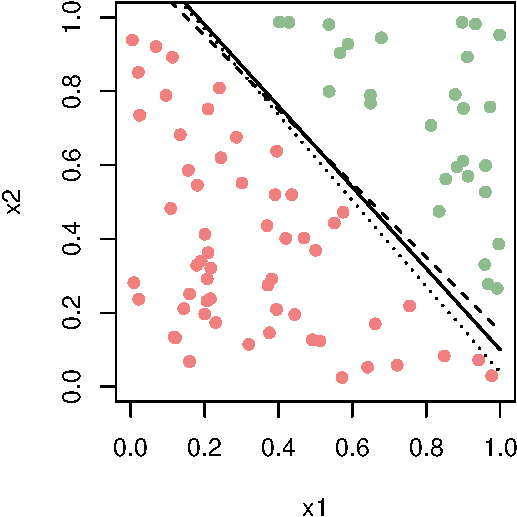
\includegraphics{9SVM_files/figure-latex/unnamed-chunk-6-1.pdf}

\begin{center}\rule{0.5\linewidth}{\linethickness}\end{center}

The three lines displayed in the figure are three possible separating
hyperplanes for this dataset which contains two predictors \(x_1\) and
\(x_2\) (\(p=2\)). The hyperplanes have the property that

\[\beta_0+\beta_1 x_{i1} + \beta_2 x_{i2}+...+\beta_p x_{ip}=\beta_0+{\bf x}_i^T {\boldsymbol \beta}>0\]

if \(y_i=1\) (green points) and

\[\beta_0+\beta_1 x_{i1} + \beta_2 x_{i2}+...+\beta_p x_{ip}=\beta_0+{\bf x}_i^T {\boldsymbol \beta}<0\]

if \(y_i=-1\) (orange points).

\begin{center}\rule{0.5\linewidth}{\linethickness}\end{center}

This means that for all observations (all are correctly classified)
\[y_i (\beta_0+{\bf x}_i^T {\boldsymbol \beta})>0\]

The hyperplane leads to a natural classifier:

We can assign a class to a new observation depending on which side of
the hyperplane it is located. We denote the new observation
\(x^*=(x_1^*,...,x_n^*)\) and classify it as \(y^*=1\) if
\[f(x^*)=\beta_0+\beta_1 x_1^* + \beta_2 x_{2}^*+...+\beta_p x_{p}^*>0\]
and as \(y^*=-1\) otherwise.

\begin{center}\rule{0.5\linewidth}{\linethickness}\end{center}

The next question is which hyperplane we should choose.

In the above figure we plotted three possible hyperplanes, but there
exist infinitely many possible separating hyperplanes for this dataset.

A natural choice is the \textbf{maximal margin hyperplane}. This is the
separating hyperplane that is farthest from the training observations.

(From a statistical point of view we might be afraid that we are
overfitting the data now.)

\begin{center}\rule{0.5\linewidth}{\linethickness}\end{center}

\#\#Optimization problem

\begin{itemize}
\tightlist
\item
  The maximal margin hyperplane is found by computing the perpendicular
  distance from each training observation to a given separating
  hyperplane.
\item
  The smallest such distance is the minimal distance from the
  observations to the hyperplane, also known as the margin. (See
  illustration below.)
\item
  We want to maximize this margin.
\end{itemize}

\begin{center}\rule{0.5\linewidth}{\linethickness}\end{center}

\begin{figure}
\centering
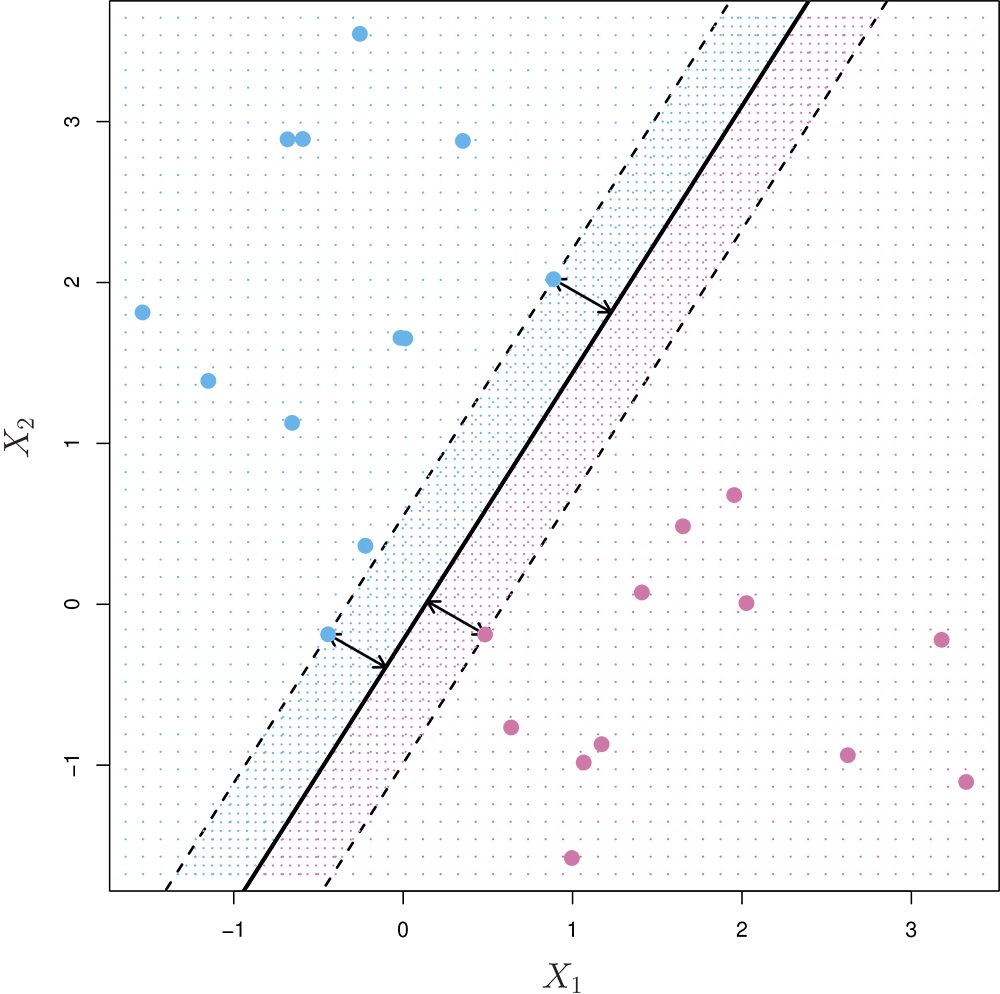
\includegraphics{../ISLR/Chapter9/9.3.png}
\caption{ISLR Figure 9.3}
\end{figure}

\begin{center}\rule{0.5\linewidth}{\linethickness}\end{center}

The process of finding the maximal margin hyperplane for a dataset with
\(p\) covariates and \(n\) training observations can be formulated
through the following optimization problem:

\[\mathrm{maximize}_{\beta_0,\beta_1,...,\beta_p} \quad M \]
\[\text{subject to} \sum_{j=1}^p \beta_j^2=1,\]
\[y_i(\beta_0+\beta_1 x_{i1}+\beta_2 x_{i2}+...+\beta_p x_{ip})\geq M \quad  \forall i=1,...,n\]
where \(M\) is the width of the margin.

Observe: \(y_i(\beta_0+{\bf x}^T {\boldsymbol \beta})\) is the (signed)
distance from the \(i\)th point to the hyperplane defined by the
\(\beta\)s. We want to find the hyperplane, where each observaton is at
least \(M\) units away - on the correct side, where \(M\) is as big as
possible.

\begin{center}\rule{0.5\linewidth}{\linethickness}\end{center}

Above (Figure 9.3. from James et al. (2013)) three of the observations
are equidistant from the hyperplane. These are called \textbf{support
vectors}. If one of the support vectors changes its position, the whole
hyperplane will move. This is a property of the maximal margin
hyperplane: It only depends on the support vectors, and not on the other
observations.

\begin{center}\rule{0.5\linewidth}{\linethickness}\end{center}

It can be shown, see for example Efron and Hastie (2016) Section 19.1
and Friedman, Hastie, and Tibshirani (2001) Section 4.5, that the
optimization problem can be reformulated using Lagrange multipliers
(primal and dual problem) into a quadratic convex optimization problem
that can be solved efficiently.

However, we do of cause have to solve the optimization problem to
identify the support vectors and the unknown parameters for the
separating hyperplane.

Since we in TMA4268 Statistical learning do not require a course in
optimization - we do not go into details here.

\begin{center}\rule{0.5\linewidth}{\linethickness}\end{center}

\hypertarget{questions}{%
\subsection{Questions}\label{questions}}

\begin{itemize}
\tightlist
\item
  Explain briefly the idea behind the maximal margin classifier.
\item
  Is there any tuning parameters that need to be chosen?
\item
  What if our problem is not separable by a hyperplane?
\end{itemize}

\begin{center}\rule{0.5\linewidth}{\linethickness}\end{center}

\textbf{A}:

MMC: drawing is the best! Hyperplane with largest possible margin to the
support vectors, all training data correctly classified (since separable
problem). Only support vectors decide boundary. No distribution assumed
for the observations in each class.

No tuning parameter.

Non-separable case is next - by defining slack-variables.

\begin{center}\rule{0.5\linewidth}{\linethickness}\end{center}

\#Support Vector Classifiers

For some data sets a separating hyperplane does not exist, the data set
is \emph{non-separable}.

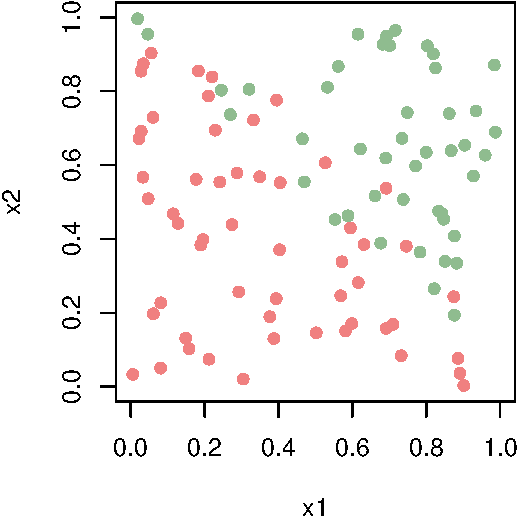
\includegraphics{9SVM_files/figure-latex/unnamed-chunk-9-1.pdf}

It is still possible to construct a hyperplane and use it for
classification, but then we have to allow some of the training
observations to be misclassified.

\begin{center}\rule{0.5\linewidth}{\linethickness}\end{center}

Also, in some situation we what to allow for some misclassifications to
make the class boundaries more robust to future observations - that is,
we have noisy data or outliers are present.

In the special case where we have more predictors than observations it
is possible to find a separating hyperplane, but the might not be the
``best'' hyperplane for us.

We now relax the maximal margin classifier to allow for a
\emph{soft-margin classifier}.

\begin{center}\rule{0.5\linewidth}{\linethickness}\end{center}

\hypertarget{optimization-problem}{%
\subsection{Optimization problem}\label{optimization-problem}}

\[\mathrm{maximize}_{\beta_0,\beta_1,...,\beta_p,\epsilon_1,...,\epsilon_n,} \quad M \text{ subject to} \sum_{j=1}^p \beta_j^2=1\]
\[y_i(\beta_0+\beta_1 x_{i1}+\beta_2 x_{i2}+...+\beta_p x_{ip})\geq M(1-\epsilon_i) \quad  \forall i=1,...,n.\]
\[\epsilon_i\geq 0, \quad \sum_{i=1}^n \epsilon_i \leq C.\]

\begin{center}\rule{0.5\linewidth}{\linethickness}\end{center}

\begin{itemize}
\tightlist
\item
  \(M\) is the width of the margin.
\item
  \(\epsilon_1,...,\epsilon_n\) are \emph{slack variables}.

  \begin{itemize}
  \tightlist
  \item
    If \(\epsilon_i=0\) it means that observation \(i\) is on the
    correct side of the margin,
  \item
    if \(\epsilon_i>0\) observation \(i\) is on the wrong side of the
    margin, and
  \item
    if \(\epsilon_i>1\) observation \(i\) is on the wrong side of the
    hyperplane.
  \end{itemize}
\item
  \(C\) is a \emph{tuning (regularization) parameter} (chosen by
  cross-validation) giving the \emph{budget for slacks}. It restricts
  the number of the training observations that can be on the wrong side
  of the hyperplane. No more than \(C\) of the observations can be on
  the wrong side.
\end{itemize}

\begin{center}\rule{0.5\linewidth}{\linethickness}\end{center}

The hyperplane has the property that it \textbf{only} depends on the
observations that \textbf{either lie on the margin or on the wrong side
of the margin}.

These observations are called our \textbf{support vectors}. The
observations on the correct side of the margin do not affect the support
vectors. The length of distance for the support vectors to the class
boundary is proportional to the slacks.

\begin{center}\rule{0.5\linewidth}{\linethickness}\end{center}

\textbf{Classification rule:} We classify a test observation
\({\bf x}^*\) based on the sign of
\(f({\bf x}^*)=\beta_0+\beta_1 x_1^*+...+\beta_p x_p^*\) as before:

\begin{itemize}
\tightlist
\item
  If \(f({\bf x}^*)<0\) then \(y^*=-1\).
\item
  If \(f({\bf x}^*)>0\) then \(y^*=1\).
\end{itemize}

More on solving the optimization problem: Friedman, Hastie, and
Tibshirani (2001) Section 12.2.1 (primal and dual Lagrange problem,
quadratic convex problem).

\begin{center}\rule{0.5\linewidth}{\linethickness}\end{center}

\hypertarget{questions-1}{%
\subsection{Questions}\label{questions-1}}

\begin{itemize}
\tightlist
\item
  Should the variables be standardized before used with this method?
\item
  The support vector classifier only depends on the observations that
  violate the margin. How does \(C\) affect the width of the margin?\\
\item
  Discuss how the tuning parameter \(C\) affects the bias-variance
  trade-off of the method.
\end{itemize}

\begin{center}\rule{0.5\linewidth}{\linethickness}\end{center}

\begin{figure}
\centering
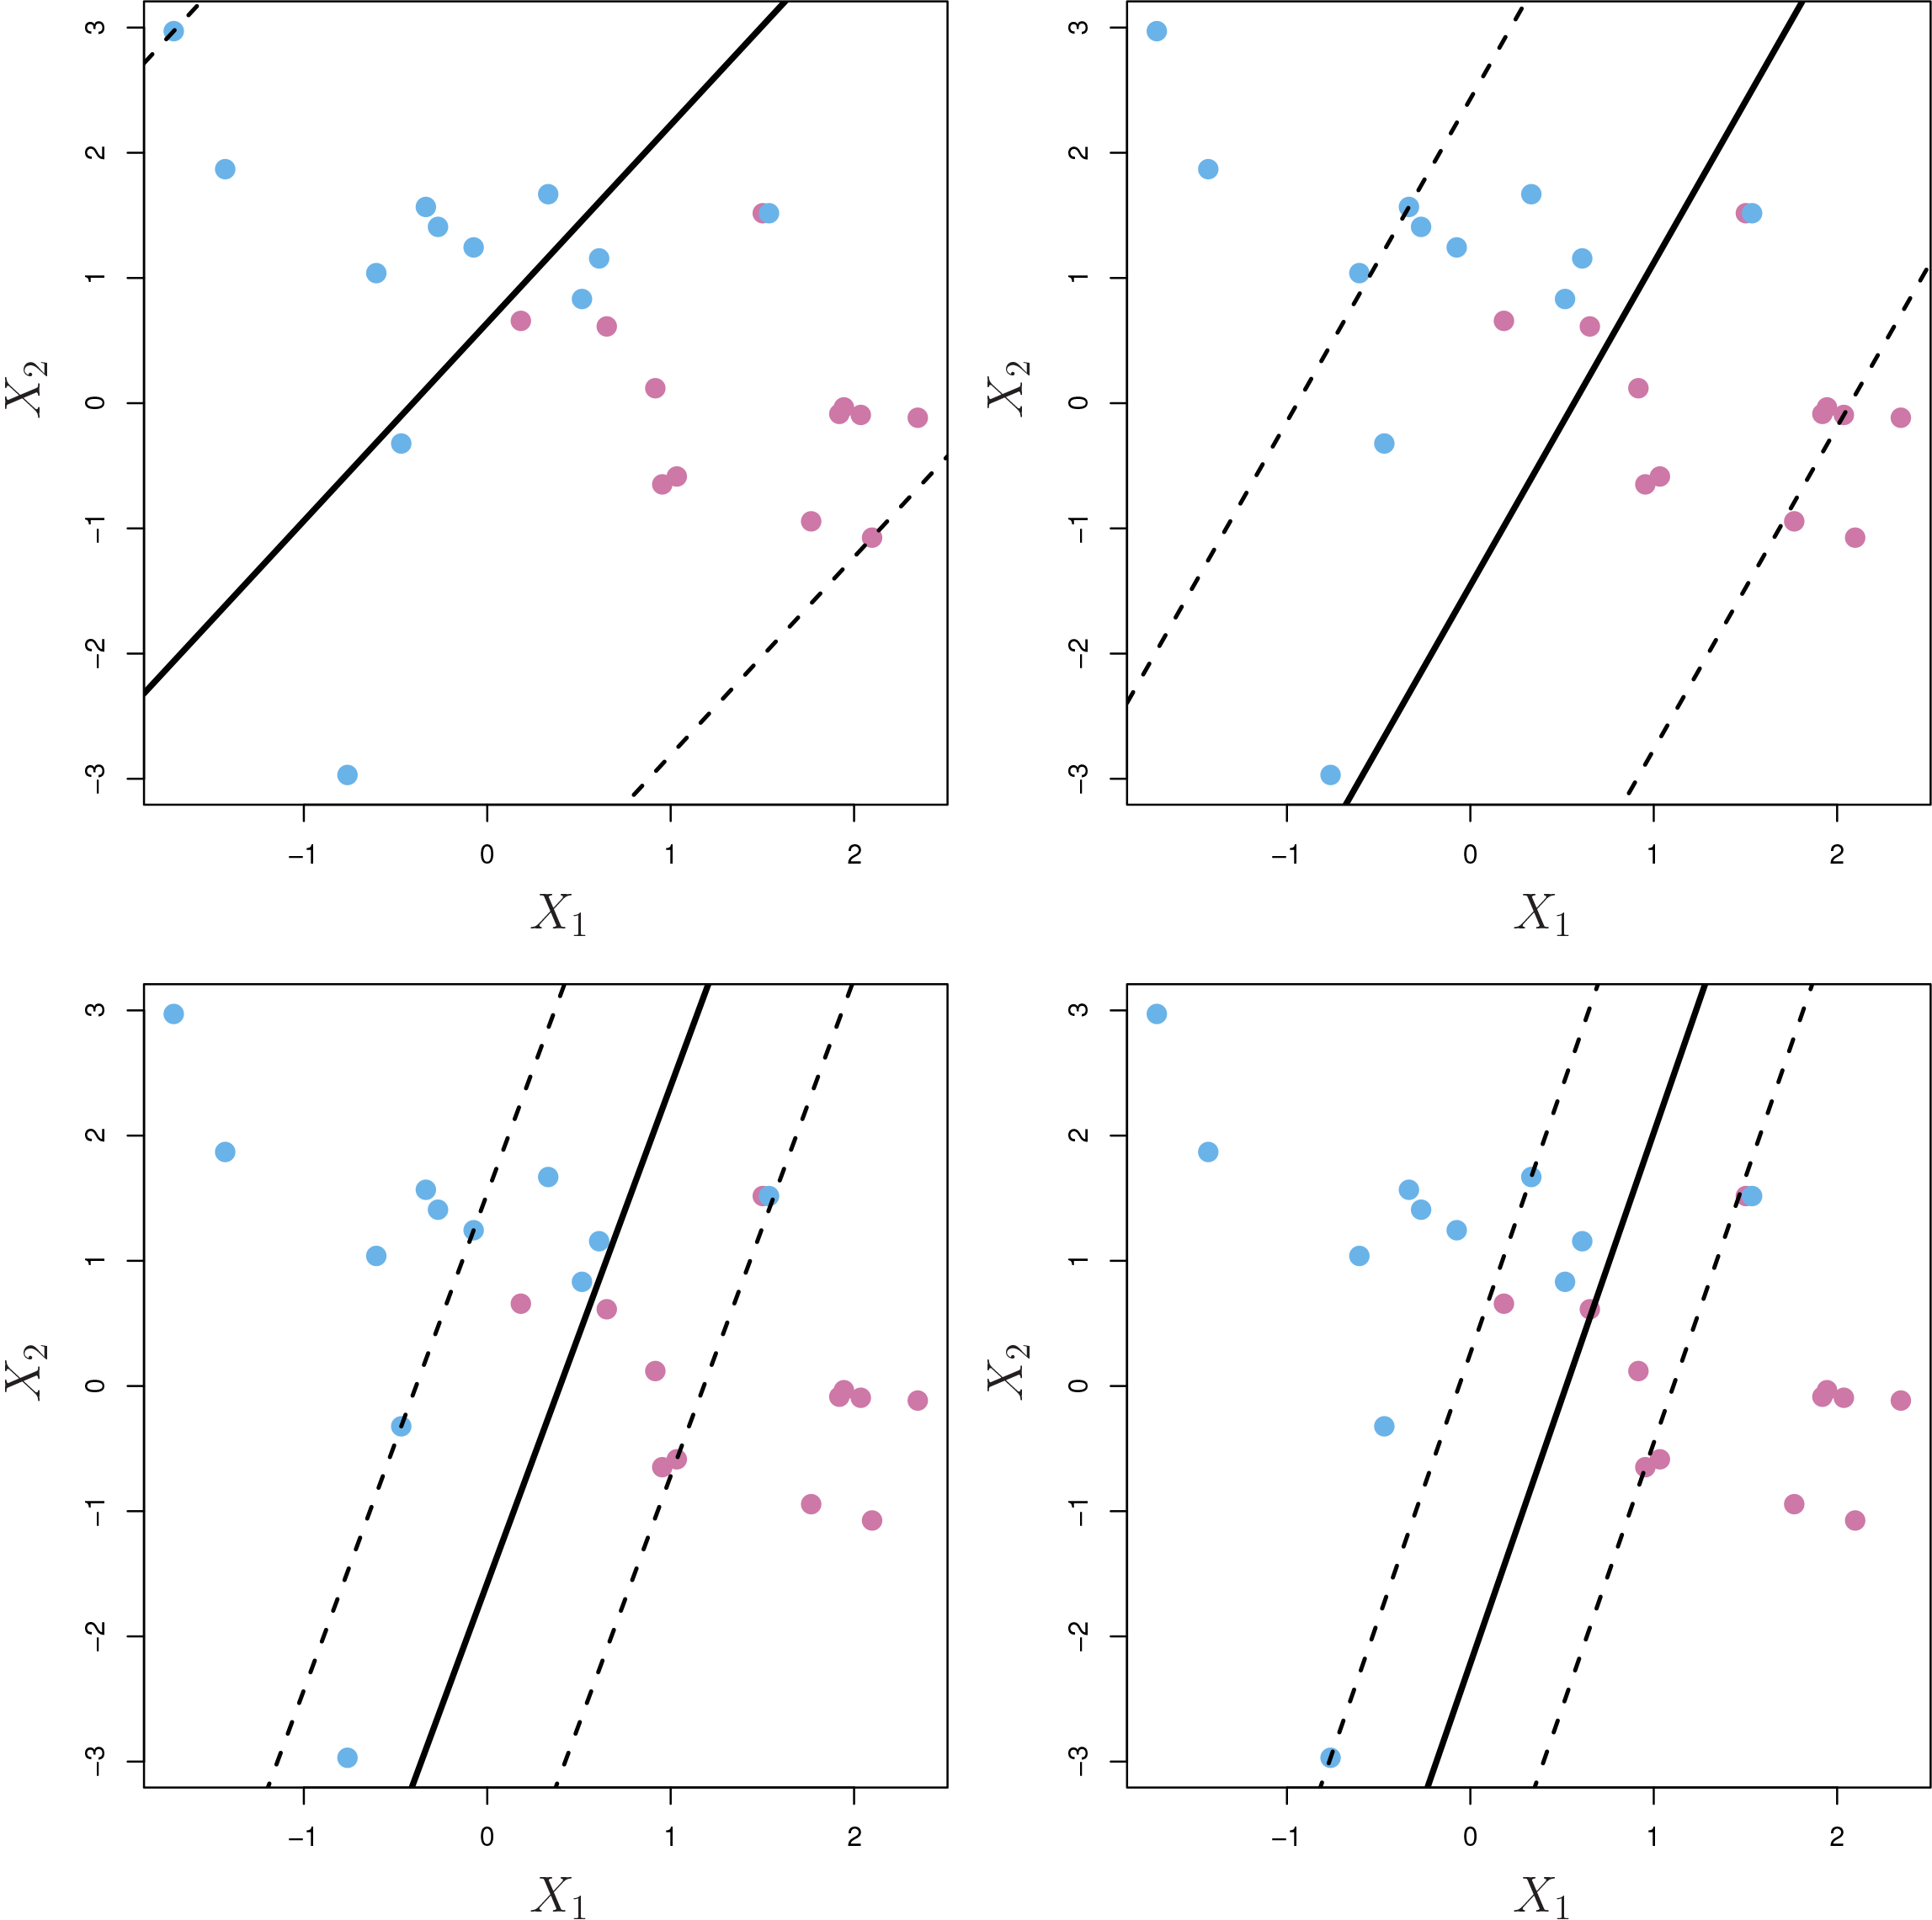
\includegraphics{../ISLR/Chapter9/9.7.png}
\caption{ISLR Figure 9.7: Top left=large C, smaller top right, bottom
left and bottom right. As C decreases the tolerance for observations
being on the wrong side of the margin decreases and the marin narrows.}
\end{figure}

See also Figure 19.3 in Efron and Hastie (2016).

\begin{center}\rule{0.5\linewidth}{\linethickness}\end{center}

\textbf{A:} Yes, should be standardized because this method treats all
variables equally. Same as for lasso and ridge.

If \(C\) is small then \(M\) must give narrow margin? \(C\) is our
bias-variance trade-off tuning parameter: C large: allow many
violations: more bias, less variance. C small: highly fit the data: less
bias, more variance.

\begin{center}\rule{0.5\linewidth}{\linethickness}\end{center}

\#\#Example\#\# We will now find a support vector classifier for the
second training dataset (forest2) and use this to classify the
observations in the second test set (seeds2).

\begin{itemize}
\tightlist
\item
  There are \(100\) observations of trees: 45 pines (\(y_i=1\)) and 55
  redwood trees (\(y_i=-1\)).
\item
  In the test set there are 20 seeds: 10 pine seeds and 10 redwood
  seeds.
\end{itemize}

The function \texttt{svm} in the package \texttt{e1071} is used to find
the maximal margin hyperplane. The response needs to be coded as a
factor variable, and the data set has to be stored as a dataframe.

\footnotesize

\begin{Shaded}
\begin{Highlighting}[]
\KeywordTok{library}\NormalTok{(e1071)}
\NormalTok{forest2 =}\StringTok{ }\KeywordTok{read.table}\NormalTok{(}\DataTypeTok{file =} \StringTok{"https://www.math.ntnu.no/emner/TMA4268/2019v/data/forest2.txt"}\NormalTok{)}
\NormalTok{seeds2 =}\StringTok{ }\KeywordTok{read.table}\NormalTok{(}\DataTypeTok{file =} \StringTok{"https://www.math.ntnu.no/emner/TMA4268/2019v/data/seeds2.txt"}\NormalTok{)}
\NormalTok{train2 =}\StringTok{ }\KeywordTok{data.frame}\NormalTok{(}\DataTypeTok{x =}\NormalTok{ forest2[, }\DecValTok{1}\OperatorTok{:}\DecValTok{2}\NormalTok{], }\DataTypeTok{y =} \KeywordTok{as.factor}\NormalTok{(forest2[, }\DecValTok{3}\NormalTok{]))}
\NormalTok{test2 =}\StringTok{ }\KeywordTok{data.frame}\NormalTok{(}\DataTypeTok{x =}\NormalTok{ seeds2[, }\DecValTok{1}\OperatorTok{:}\DecValTok{2}\NormalTok{], }\DataTypeTok{y =} \KeywordTok{as.factor}\NormalTok{(seeds2[, }\DecValTok{3}\NormalTok{]))}
\end{Highlighting}
\end{Shaded}

\normalsize

\begin{center}\rule{0.5\linewidth}{\linethickness}\end{center}

The \texttt{svm} function uses a slightly different formulation from
what we wrote above.

We had in our presentation a budget for errors \(C\), but in
\texttt{svm} we instead have an argument \texttt{cost} that allows us to
specify the cost of violating the margin.

\begin{itemize}
\tightlist
\item
  When \texttt{cost} is set to a low value, the margin will be wider
  than if set to a large value.
\end{itemize}

We first try with \texttt{cost=1}. We set
\texttt{kernel=\textquotesingle{}linear\textquotesingle{}} as we are
interested in a linear decision boundary. \texttt{scale=TRUE} scales the
predictors to have mean 0 and standard deviation 1. We choose not to
scale.

\begin{center}\rule{0.5\linewidth}{\linethickness}\end{center}

\footnotesize

\begin{Shaded}
\begin{Highlighting}[]
\NormalTok{svmfit_linear1 =}\StringTok{ }\KeywordTok{svm}\NormalTok{(y }\OperatorTok{~}\StringTok{ }\NormalTok{., }\DataTypeTok{data =}\NormalTok{ train2, }\DataTypeTok{kernel =} \StringTok{"linear"}\NormalTok{, }\DataTypeTok{cost =} \DecValTok{1}\NormalTok{, }
    \DataTypeTok{scale =} \OtherTok{FALSE}\NormalTok{)}
\KeywordTok{plot}\NormalTok{(svmfit_linear1, train2, }\DataTypeTok{col =} \KeywordTok{c}\NormalTok{(}\StringTok{"lightcoral"}\NormalTok{, }\StringTok{"lightgreen"}\NormalTok{))}
\end{Highlighting}
\end{Shaded}

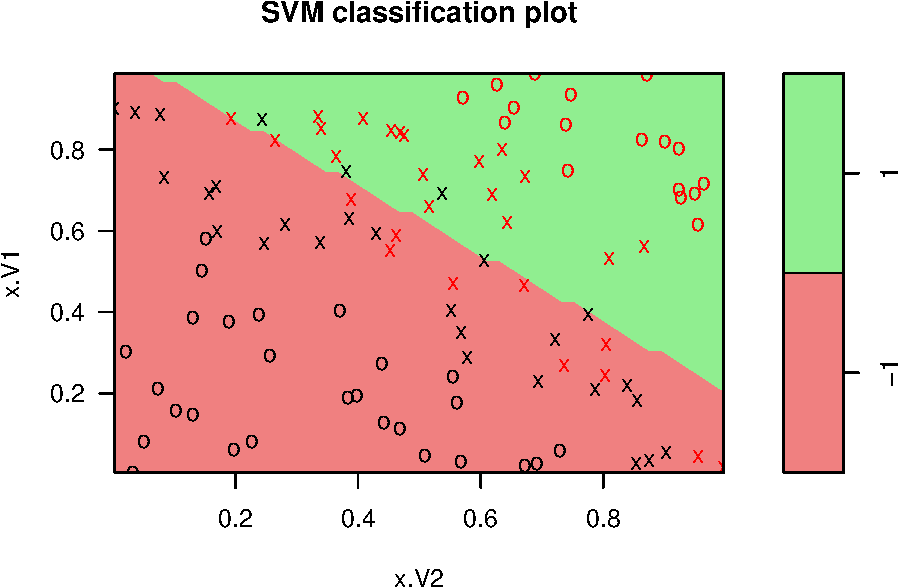
\includegraphics{9SVM_files/figure-latex/unnamed-chunk-11-1.pdf}

\begin{center}\rule{0.5\linewidth}{\linethickness}\end{center}

\begin{Shaded}
\begin{Highlighting}[]
\KeywordTok{summary}\NormalTok{(svmfit_linear1)}
\end{Highlighting}
\end{Shaded}

\begin{verbatim}
## 
## Call:
## svm(formula = y ~ ., data = train2, kernel = "linear", cost = 1, 
##     scale = FALSE)
## 
## 
## Parameters:
##    SVM-Type:  C-classification 
##  SVM-Kernel:  linear 
##        cost:  1 
## 
## Number of Support Vectors:  56
## 
##  ( 28 28 )
## 
## 
## Number of Classes:  2 
## 
## Levels: 
##  -1 1
\end{verbatim}

\begin{Shaded}
\begin{Highlighting}[]
\NormalTok{svmfit_linear1}\OperatorTok{$}\NormalTok{index  }\CommentTok{#support vectors id in data set}
\end{Highlighting}
\end{Shaded}

\begin{verbatim}
##  [1]  1  2  4  6  9 10 16 21 26 27 28 40 44 53 55 57 58 65 67 72 76 77 80
## [24] 81 87 91 92 98  5  8 11 13 18 19 20 23 24 25 34 36 39 41 42 47 48 59
## [47] 61 62 70 71 75 78 88 93 95 96
\end{verbatim}

\normalsize

\begin{center}\rule{0.5\linewidth}{\linethickness}\end{center}

\textbf{Observations}

\begin{itemize}
\tightlist
\item
  Remark that the \(x_1\) is plotted on the vertical axis, and the the
  implementation of the plotting function is made in a way that the
  linear boundary looks jagged.
\item
  The crosses in the plot indicate the support vectors. With \(cost=1\),
  we have 56 support vectors, 28 in each class.
\item
  All other observations are shown as circles.
\end{itemize}

\begin{center}\rule{0.5\linewidth}{\linethickness}\end{center}

Next, we set \(cost=100\): \footnotesize

\begin{Shaded}
\begin{Highlighting}[]
\NormalTok{svmfit_linear2 =}\StringTok{ }\KeywordTok{svm}\NormalTok{(y }\OperatorTok{~}\StringTok{ }\NormalTok{., }\DataTypeTok{data =}\NormalTok{ train2, }\DataTypeTok{kernel =} \StringTok{"linear"}\NormalTok{, }\DataTypeTok{cost =} \DecValTok{100}\NormalTok{, }
    \DataTypeTok{scale =} \OtherTok{FALSE}\NormalTok{)}
\KeywordTok{plot}\NormalTok{(svmfit_linear2, train2, }\DataTypeTok{col =} \KeywordTok{c}\NormalTok{(}\StringTok{"lightcoral"}\NormalTok{, }\StringTok{"lightgreen"}\NormalTok{))}
\end{Highlighting}
\end{Shaded}

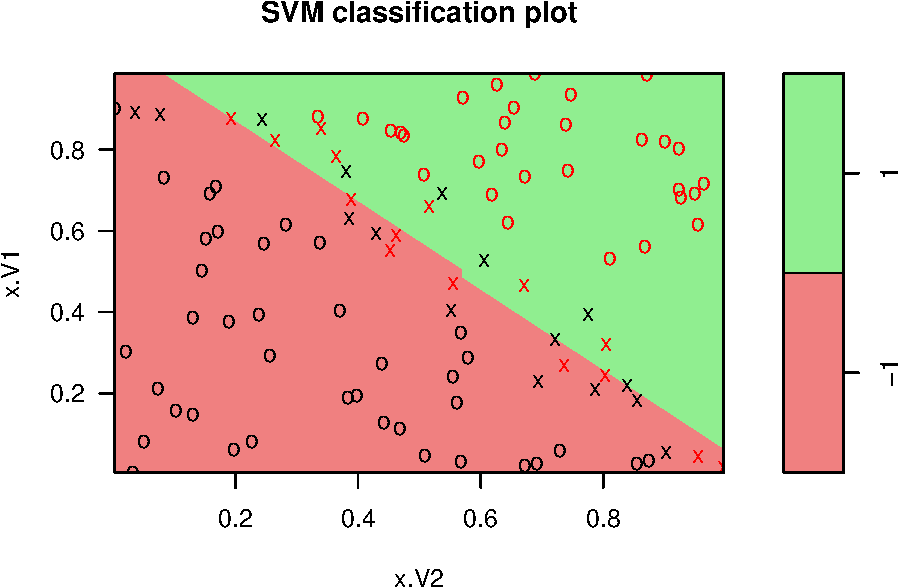
\includegraphics{9SVM_files/figure-latex/unnamed-chunk-13-1.pdf}

\begin{center}\rule{0.5\linewidth}{\linethickness}\end{center}

\begin{Shaded}
\begin{Highlighting}[]
\KeywordTok{summary}\NormalTok{(svmfit_linear2)}
\end{Highlighting}
\end{Shaded}

\begin{verbatim}
## 
## Call:
## svm(formula = y ~ ., data = train2, kernel = "linear", cost = 100, 
##     scale = FALSE)
## 
## 
## Parameters:
##    SVM-Type:  C-classification 
##  SVM-Kernel:  linear 
##        cost:  100 
## 
## Number of Support Vectors:  31
## 
##  ( 15 16 )
## 
## 
## Number of Classes:  2 
## 
## Levels: 
##  -1 1
\end{verbatim}

\normalsize

\begin{center}\rule{0.5\linewidth}{\linethickness}\end{center}

With \(cost=100\) we have 31 support vectors, i.e the width of the
margin is decreased.

How do we find an optimal \(cost\) parameter? By using the \emph{tune()}
function we can perform ten-fold cross-validation and find the
cost-parameter that gives the lowest cross-validation error:

\footnotesize

\begin{Shaded}
\begin{Highlighting}[]
\KeywordTok{set.seed}\NormalTok{(}\DecValTok{1}\NormalTok{)}
\NormalTok{CV_linear =}\StringTok{ }\KeywordTok{tune}\NormalTok{(svm, y }\OperatorTok{~}\StringTok{ }\NormalTok{., }\DataTypeTok{data =}\NormalTok{ train2, }\DataTypeTok{kernel =} \StringTok{"linear"}\NormalTok{, }\DataTypeTok{ranges =} \KeywordTok{list}\NormalTok{(}\DataTypeTok{cost =} \KeywordTok{c}\NormalTok{(}\FloatTok{0.001}\NormalTok{, }
    \FloatTok{0.01}\NormalTok{, }\FloatTok{0.1}\NormalTok{, }\DecValTok{1}\NormalTok{, }\DecValTok{5}\NormalTok{, }\DecValTok{10}\NormalTok{, }\DecValTok{100}\NormalTok{)))}
\KeywordTok{summary}\NormalTok{(CV_linear)}
\end{Highlighting}
\end{Shaded}

\begin{verbatim}
## 
## Parameter tuning of 'svm':
## 
## - sampling method: 10-fold cross validation 
## 
## - best parameters:
##  cost
##     5
## 
## - best performance: 0.14 
## 
## - Detailed performance results:
##    cost error dispersion
## 1 1e-03  0.45 0.10801234
## 2 1e-02  0.23 0.12516656
## 3 1e-01  0.16 0.11737878
## 4 1e+00  0.15 0.10801234
## 5 5e+00  0.14 0.10749677
## 6 1e+01  0.15 0.09718253
## 7 1e+02  0.15 0.09718253
\end{verbatim}

\normalsize

\begin{center}\rule{0.5\linewidth}{\linethickness}\end{center}

According to the \emph{tune()} function we should set the cost parameter
to 0.1. The function also stores the best model obtained and we can
access it as follows:

\begin{Shaded}
\begin{Highlighting}[]
\NormalTok{bestmod_linear =}\StringTok{ }\NormalTok{CV_linear}\OperatorTok{$}\NormalTok{best.model}
\end{Highlighting}
\end{Shaded}

Next, we want to predict the class label of the seeds in the test set.
We use the \texttt{predict} function and make a confusion table:

\begin{Shaded}
\begin{Highlighting}[]
\NormalTok{ypred_linear =}\StringTok{ }\KeywordTok{predict}\NormalTok{(bestmod_linear, test2)}
\KeywordTok{table}\NormalTok{(}\DataTypeTok{predict =}\NormalTok{ ypred_linear, }\DataTypeTok{truth =}\NormalTok{ test2[, }\DecValTok{3}\NormalTok{])}
\end{Highlighting}
\end{Shaded}

\begin{verbatim}
##        truth
## predict -1  1
##      -1  8  0
##      1   2 10
\end{verbatim}

\begin{center}\rule{0.5\linewidth}{\linethickness}\end{center}

\footnotesize

\begin{Shaded}
\begin{Highlighting}[]
\KeywordTok{par}\NormalTok{(}\DataTypeTok{mfrow =} \KeywordTok{c}\NormalTok{(}\DecValTok{1}\NormalTok{, }\DecValTok{2}\NormalTok{))}
\KeywordTok{par}\NormalTok{(}\DataTypeTok{pty =} \StringTok{"s"}\NormalTok{)}
\KeywordTok{plot}\NormalTok{(}\OtherTok{NA}\NormalTok{, }\DataTypeTok{xlab =} \StringTok{"x1"}\NormalTok{, }\DataTypeTok{ylab =} \StringTok{"x2"}\NormalTok{, }\DataTypeTok{xlim =} \KeywordTok{c}\NormalTok{(}\DecValTok{0}\NormalTok{, }\DecValTok{1}\NormalTok{), }\DataTypeTok{ylim =} \KeywordTok{c}\NormalTok{(}\DecValTok{0}\NormalTok{, }\DecValTok{1}\NormalTok{))}
\KeywordTok{title}\NormalTok{(}\StringTok{"True class"}\NormalTok{)}
\KeywordTok{points}\NormalTok{(seeds2[seeds2[, }\DecValTok{3}\NormalTok{] }\OperatorTok{==}\StringTok{ }\DecValTok{-1}\NormalTok{, }\DecValTok{1}\OperatorTok{:}\DecValTok{2}\NormalTok{], }\DataTypeTok{pch =} \DecValTok{19}\NormalTok{, }\DataTypeTok{col =} \StringTok{"lightcoral"}\NormalTok{, }
    \DataTypeTok{cex =} \FloatTok{0.9}\NormalTok{)}
\KeywordTok{points}\NormalTok{(seeds2[seeds2[, }\DecValTok{3}\NormalTok{] }\OperatorTok{==}\StringTok{ }\DecValTok{1}\NormalTok{, }\DecValTok{1}\OperatorTok{:}\DecValTok{2}\NormalTok{], }\DataTypeTok{pch =} \DecValTok{19}\NormalTok{, }\DataTypeTok{col =} \StringTok{"darkseagreen"}\NormalTok{, }
    \DataTypeTok{cex =} \FloatTok{0.9}\NormalTok{)}
\KeywordTok{points}\NormalTok{(seeds2[}\KeywordTok{which}\NormalTok{(ypred_linear }\OperatorTok{!=}\StringTok{ }\NormalTok{seeds2[, }\DecValTok{3}\NormalTok{]), }\DecValTok{1}\OperatorTok{:}\DecValTok{2}\NormalTok{], }\DataTypeTok{pch =} \DecValTok{21}\NormalTok{)  }\CommentTok{#Mark misclassification.}

\KeywordTok{plot}\NormalTok{(}\OtherTok{NA}\NormalTok{, }\DataTypeTok{xlab =} \StringTok{"x1"}\NormalTok{, }\DataTypeTok{ylab =} \StringTok{"x2"}\NormalTok{, }\DataTypeTok{xlim =} \KeywordTok{c}\NormalTok{(}\DecValTok{0}\NormalTok{, }\DecValTok{1}\NormalTok{), }\DataTypeTok{ylim =} \KeywordTok{c}\NormalTok{(}\DecValTok{0}\NormalTok{, }\DecValTok{1}\NormalTok{))}
\KeywordTok{title}\NormalTok{(}\StringTok{"Predicted class"}\NormalTok{)}
\KeywordTok{points}\NormalTok{(seeds2[ypred_linear }\OperatorTok{==}\StringTok{ }\DecValTok{-1}\NormalTok{, }\DecValTok{1}\OperatorTok{:}\DecValTok{2}\NormalTok{], }\DataTypeTok{pch =} \DecValTok{19}\NormalTok{, }\DataTypeTok{col =} \StringTok{"lightcoral"}\NormalTok{, }
    \DataTypeTok{cex =} \FloatTok{0.9}\NormalTok{)}
\KeywordTok{points}\NormalTok{(seeds2[ypred_linear }\OperatorTok{==}\StringTok{ }\DecValTok{1}\NormalTok{, }\DecValTok{1}\OperatorTok{:}\DecValTok{2}\NormalTok{], }\DataTypeTok{pch =} \DecValTok{19}\NormalTok{, }\DataTypeTok{col =} \StringTok{"darkseagreen"}\NormalTok{, }
    \DataTypeTok{cex =} \FloatTok{0.9}\NormalTok{)}
\KeywordTok{points}\NormalTok{(seeds2[}\KeywordTok{which}\NormalTok{(ypred_linear }\OperatorTok{!=}\StringTok{ }\NormalTok{seeds2[, }\DecValTok{3}\NormalTok{]), }\DecValTok{1}\OperatorTok{:}\DecValTok{2}\NormalTok{], }\DataTypeTok{pch =} \DecValTok{21}\NormalTok{)  }\CommentTok{#Mark misclassification.}
\end{Highlighting}
\end{Shaded}

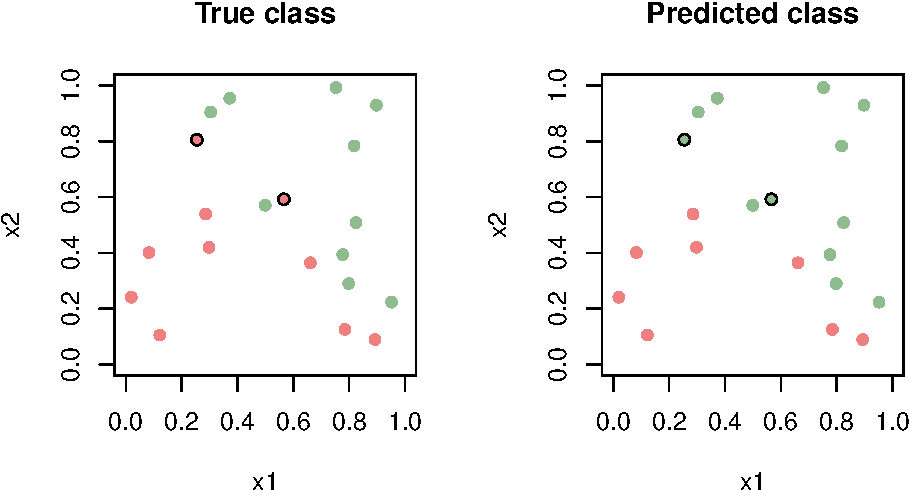
\includegraphics{9SVM_files/figure-latex/unnamed-chunk-18-1.pdf}

\normalsize

\begin{center}\rule{0.5\linewidth}{\linethickness}\end{center}

In this case three of the test observations are misclassified: These
three observations are marked with a black circle in the plot, and we
observe that they lie on the border between the green and the orange
points which is reasonable: The test observations located on the border
between green and orange are hardest to predict.

Missing: the \texttt{svm} function is not (directly) outputting the
equation for the class boundary, and not the value for the width of the
margin. Want to see how to find this? Go to the
\protect\hyperlink{recex}{recommended exercises}.

\begin{center}\rule{0.5\linewidth}{\linethickness}\end{center}

\hypertarget{support-vector-machines}{%
\section{Support Vector Machines}\label{support-vector-machines}}

For some datasets a non-linear decicion boundary between the classes is
more suitable than a linear decision boundary. In such cases you can use
a \textbf{Support Vector Machine} (SVM). This is an extension of the
support vector classifier.

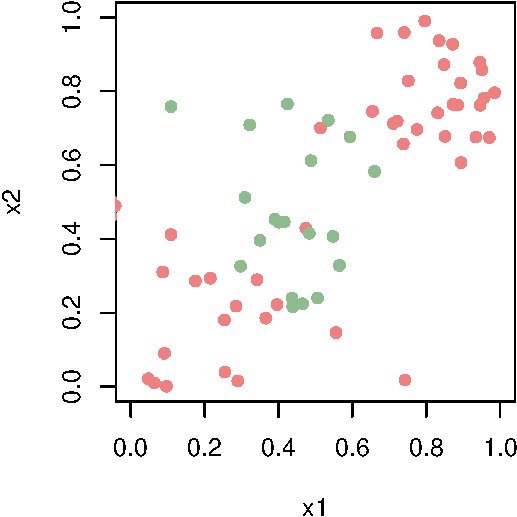
\includegraphics{9SVM_files/figure-latex/unnamed-chunk-19-1.pdf}

\begin{center}\rule{0.5\linewidth}{\linethickness}\end{center}

\hypertarget{expanding-the-feature-space}{%
\subsection{Expanding the feature
space}\label{expanding-the-feature-space}}

We saw in Module 7 that in regression we could fit non-linear curves by
using a polynomial basis - adding polynomials of different order as
covariates. This was a linear regression in the transformed variables,
but non-linear in the original variables. Maybe we may add many such
extra features and find a nice linear boundary in that high-dimensional
space?

Efron and Hastie (2016) (page 377): \emph{If \(n \le p+1\) we can always
find a separating hyperplane, unless there are exact features ties
across the class barrier.} (Two observations with equal covariate
vector, but different classes.)

\begin{center}\rule{0.5\linewidth}{\linethickness}\end{center}

\begin{figure}
\centering
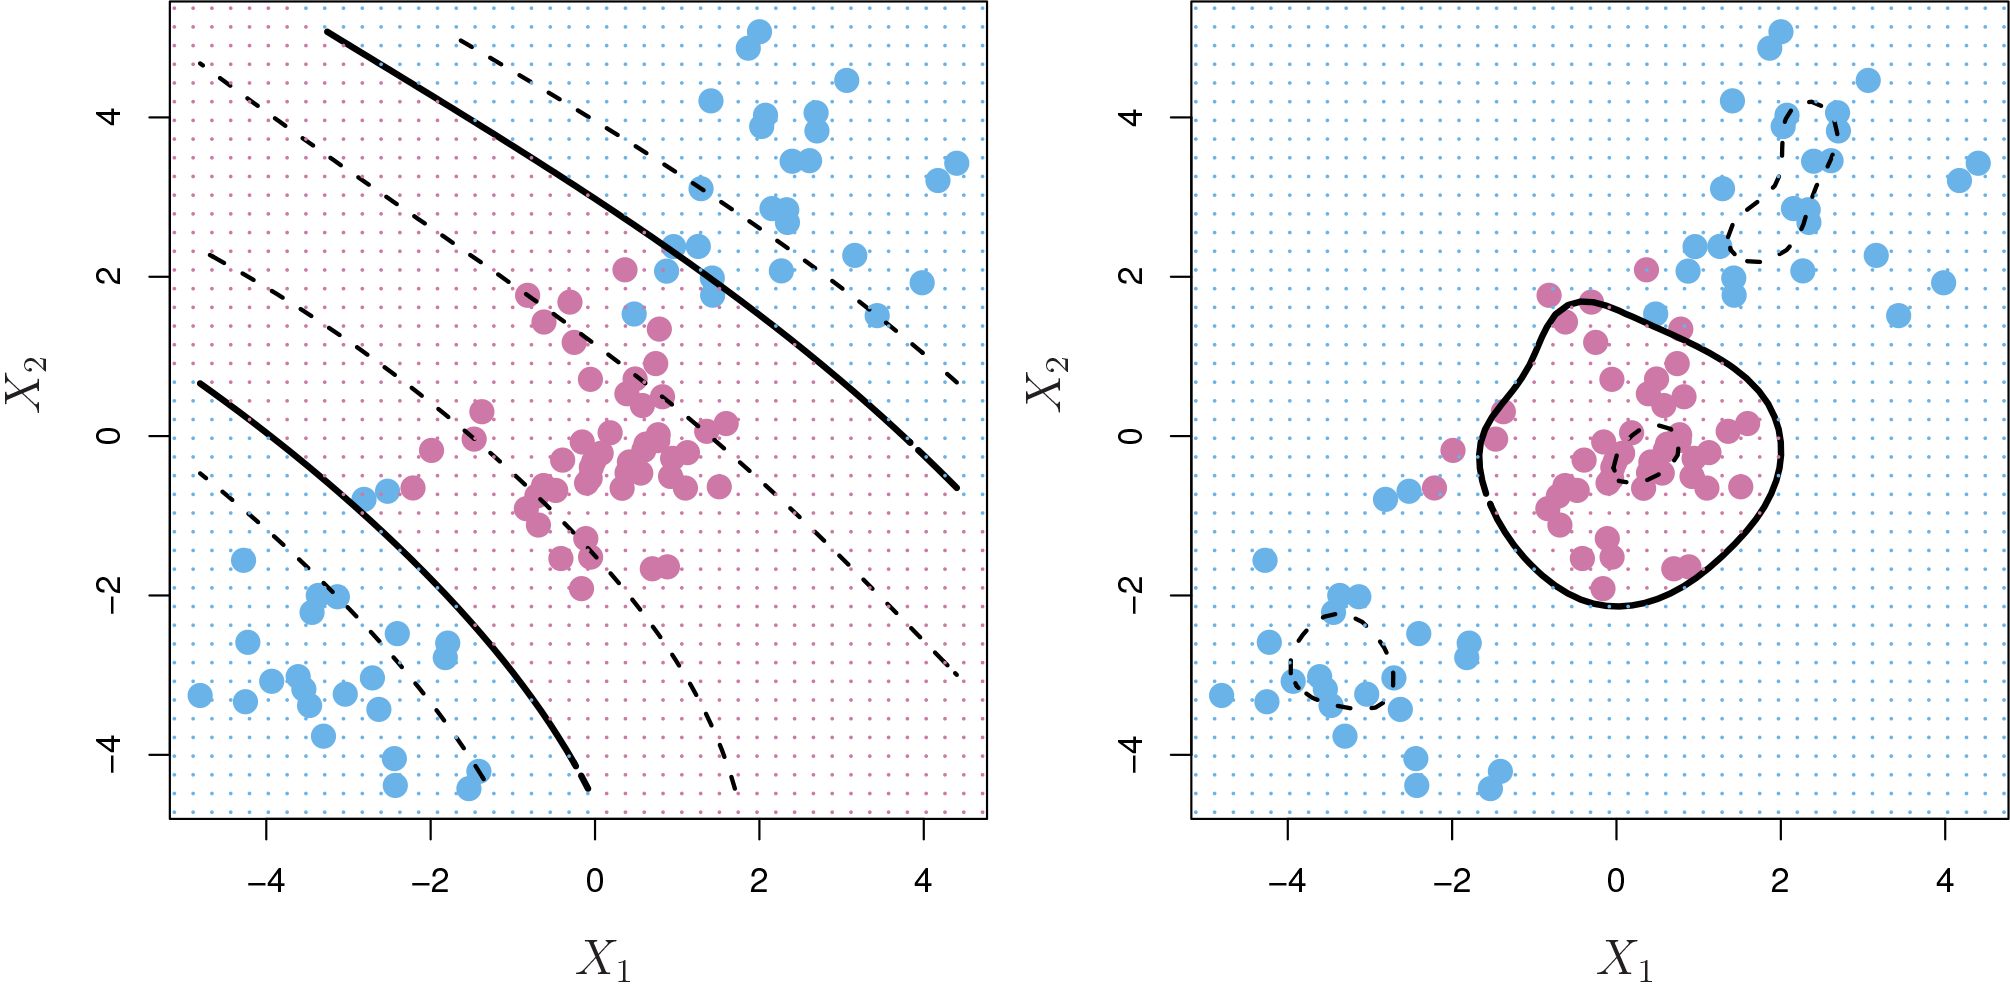
\includegraphics{../ISLR/Chapter9/9.9.png}
\caption{ISLR Figure 9.9}
\end{figure}

Left: expanding feature space to include cubic polynomials
(\(x_1,x_2,x_1x_2,x_1^2,x_2^2,x_1^2x_2,x_1x_2^2x_1^3,x_2^3\), 9
parameters to estimate in addition to intercept), and also observe the
margins. (Right: radial basis function kernel - wait a bit.)

Next: replace polynomials with \emph{kernels} for elegance and
computational issues.

\begin{center}\rule{0.5\linewidth}{\linethickness}\end{center}

\hypertarget{inner-products}{%
\subsection{Inner products}\label{inner-products}}

We have not focused on how to solve the optimisation problem of finding
the support vector classifier hyperplane, because this is outside the
scope of this course.

Remember that we classify a new observation \({\bf x}^*\) by first
calculating a numerical value for the estimated \(f({\bf x}^*)\) and
then if \(f({\bf x}^*)<0\) classify as \(-1\) and if \(f({\bf x}^*)>0\)
classify as \(1\).

It can be \emph{shown} (using optimization theory) that the solution to
the support vector classifier problem at a new observation
\({\bf x}^*\), can be expressed as \[
f({\bf x}^*)=\beta_0 + \sum_{i=1}^n \alpha_i \langle {\bf x}^*,{\bf x}_i \rangle
\] where \(\alpha_i\) is some parameter and \(i=1,...,n\).

\begin{center}\rule{0.5\linewidth}{\linethickness}\end{center}

A term of the form \(\langle {\bf x}_i, {\bf x}_{i'} \rangle\) denotes
the inner product between two observations \(i\) and \(i'\) and is
defined as: \[
\langle {\bf x}_i , {\bf x}_{i'}\rangle =\sum_{j=1}^p x_{ij} x_{i' j}.
\] This means that we need (in addition to the intercept) to estimate
\(n\) parameters (\(\alpha_i\)s) instead of \(p\) (\(\beta_j\)s) (and
for our expanded feature space then \(p\) might be larger than \(n\)).
(For the interested reader: See Eq. 19.22 and 19.23 of Efron and Hastie
(2016).)

\begin{center}\rule{0.5\linewidth}{\linethickness}\end{center}

Further, it then turns out that to estimate the parameters
\(\beta_0,\alpha_1,...,\alpha_n\) this can be based on the
\({n}\choose{2}\) inner products \(\langle {\bf x}_i,{\bf x}_i'\rangle\)
between all pair of training observations (the class of the training
observations is also included).

Also, \(\alpha_i=0\) for the observations \(i\) that are \emph{not} the
support vectors. Remark: we could alternatively say that
\(\alpha_i \neq 0\) define the support vectors.

\begin{center}\rule{0.5\linewidth}{\linethickness}\end{center}

Thus, we only need the inner product between the new observation and the
observations corresponding to support vectors to classify a new
observation, and

\[
f({\bf x})=\beta_0 + \sum_{i \in \mathcal{S}} \alpha_i \langle {\bf x}, {\bf x}_i\rangle,
\] where \(\mathcal{S}\) contains the indices of the support points. So,
we have sparsity in the observations (but not in the predictors).

\begin{center}\rule{0.5\linewidth}{\linethickness}\end{center}

\textbf{Q:} Find the support vectors

\begin{figure}
\centering
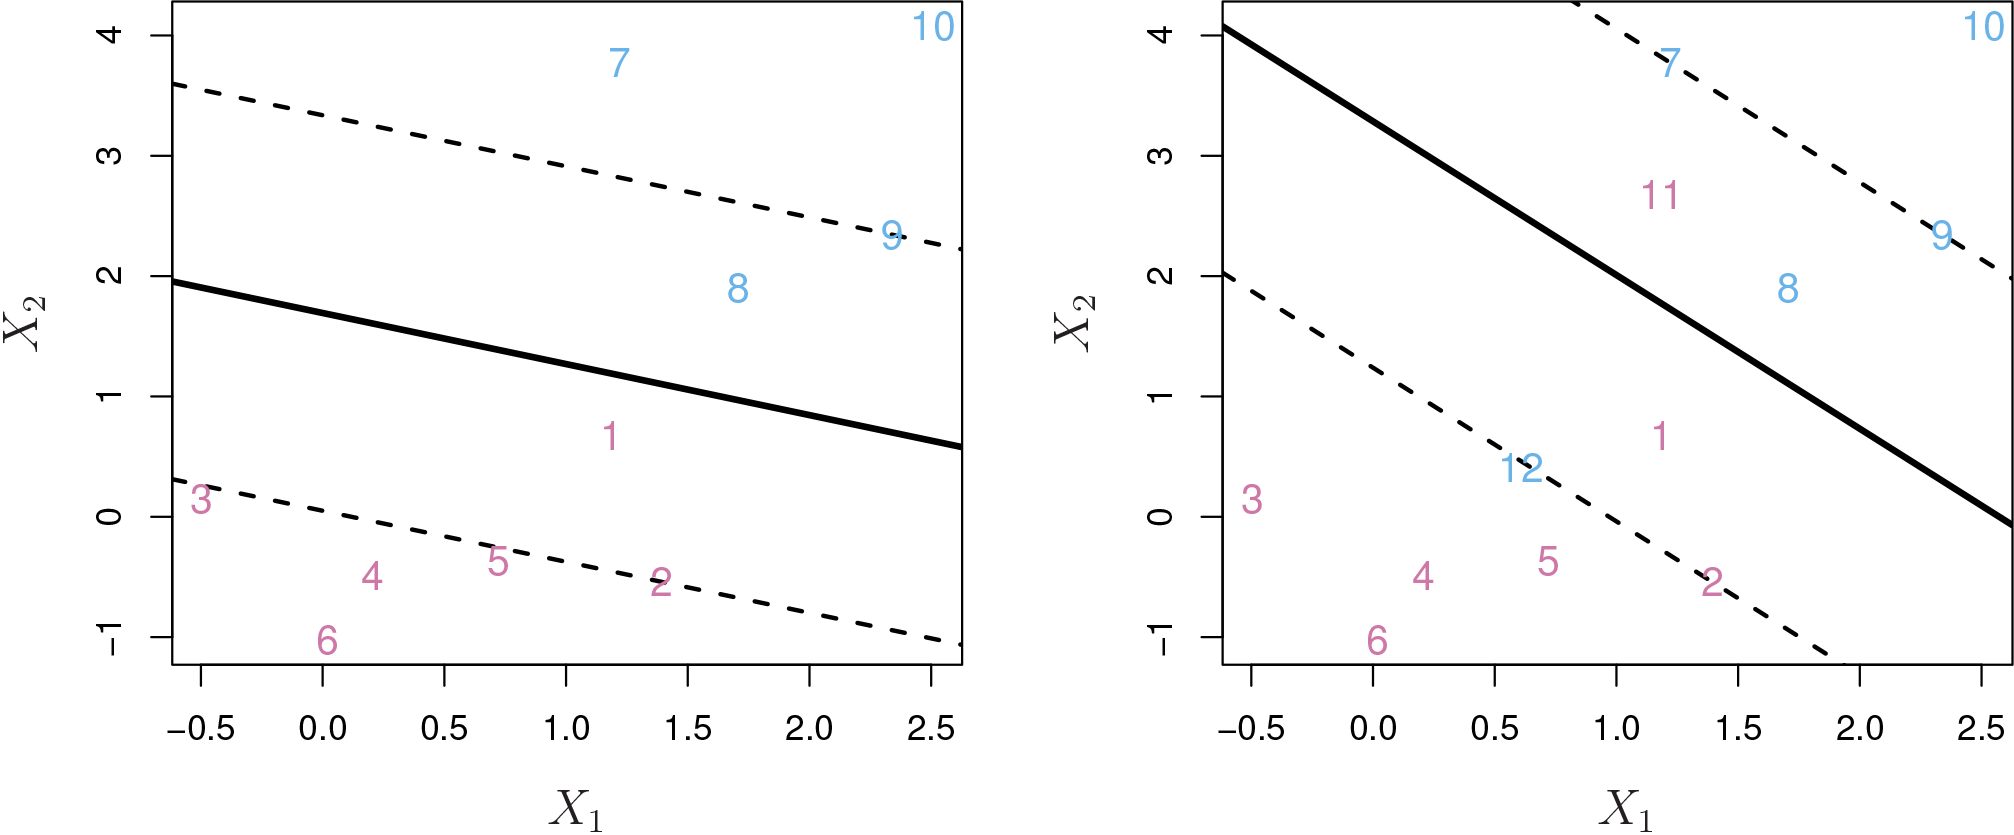
\includegraphics{../ISLR/Chapter9/9.6.png}
\caption{ISLR Figure 9.6}
\end{figure}

Observe: we need all observations (both \(x\) and \(y\) values) to
decide on which observations are the support vectors.

\begin{center}\rule{0.5\linewidth}{\linethickness}\end{center}

\hypertarget{kernels}{%
\subsection{Kernels}\label{kernels}}

(we now use \(x\) to denote a new observation)

The next step is now to \emph{replace the inner product}
\(\langle {\bf x}, {\bf x}_i\rangle\) with a function
\(K({\bf x}_i,{\bf x}_{i'})\) referred to as the \textbf{kernel}: \[
f({\bf x})=\beta_0 + \sum_{i \in \mathcal{S}} \alpha_i K({\bf x},{\bf x}_i).
\] For the linear case (which is what we have considered so far), the
kernel is simply the inner product
\(K({\bf x}_i,{\bf x}_i')=\sum_{j=1}^p x_{ij}x_{i'j}\).

The two arguments to the kernel are two \(p\)-vectors.

If we want a more flexible decision boundary we could instead use a
\textbf{polynomial kernel}. This polynomial kernel of degree \(d>1\) is
given by: \[
K({\bf x}_i,{\bf x}_i')=(1+\sum_{j1}^p x_{ij} x_{i'j})^d.
\] (This kernel is not so much used in practice, but is popular for
proofs.)

\begin{center}\rule{0.5\linewidth}{\linethickness}\end{center}

Using these kernels our solution for the class boundary can be written
of the form

\[f({\bf x})=\beta_0 +\sum_{i\in \cal{S}} \alpha_i K({\bf x},{\bf x}_i)\]

The nice thing here is that we only need to calculate the kernels, not
the basis functions (what we in Module 7 did as extra columns of the
design matrix).

\begin{center}\rule{0.5\linewidth}{\linethickness}\end{center}

A very popular choice is the radial kernel, \[
K({\bf x}_i,{\bf x}_i')=\exp(-\gamma \sum_{j=1}^p (x_{ij}-x_{i'j})^2),
\] where \(\gamma\) is a positive constant (a tuning parameter).

Observe the connection to a multivariate normal density, where
\(\gamma \propto 1/\sigma^2\) (\(\sigma^2\) variance in normal
distribution). If \(\gamma\) is small (similar to large variance in the
normal distribution) the decision boundaries are smoother than for
larger \(\gamma\).

It turns out that this computes the inner product in a very high
(infinite) dimensional feature space. But, this does not give
overfitting because some of the dimensions are ``squashed down'' (but we
have the parameter \(\gamma\) and the budget parameter that we have to
decide on).

The radial kernel is convinient if we want a circular decision boundary,
and \(\gamma\) and our budget can be chosen by cross-validation.

Remark: the mathematics behind this is based on \emph{reproducing-kernel
Hilbert spaces} (see page 384 of Efron and Hastie (2016) for a glimpse
of the theory).

\begin{center}\rule{0.5\linewidth}{\linethickness}\end{center}

Study Figures 19.5 and 19.6 (page 383) in Efron and Hastie (2016) to see
how the radial kernel can make smooth functions.

\href{https://web.stanford.edu/~hastie/CASI_files/PDF/casi.pdf}{Computer
Age Statistical Inference}

\begin{center}\rule{0.5\linewidth}{\linethickness}\end{center}

\hypertarget{kernels-and-our-optimization}{%
\subsection{Kernels and our
optimization}\label{kernels-and-our-optimization}}

We now merge our optimization problem (from our support vector
classifier) with our kernel representation \(f({\bf x})\) to get the
Support Vector Machine (SVM).

\[\mathrm{maximize}_{\beta_0,\alpha_1,...,\alpha_n,\epsilon_1,...,\epsilon_n,} \quad M \]
\[y_i(f({\bf x}_i))\geq M(1-\epsilon_i) \quad  \forall i=1,...,n.\]
\[\epsilon_i\geq 0, \quad \sum_{i=1}^n \epsilon_i \leq C.\]

where
\[f({\bf x}_i)=\beta_0 +\sum_{l\in \cal{S}} \alpha_l K({\bf x}_i,{\bf x}_l)\]

\begin{center}\rule{0.5\linewidth}{\linethickness}\end{center}

\hypertarget{tuning-parameter-example}{%
\subsection{Tuning parameter example}\label{tuning-parameter-example}}

Heart data - predict heart disease from \(p=13\) predictors.

Training errors as ROC and AUC.

\begin{figure}
\centering
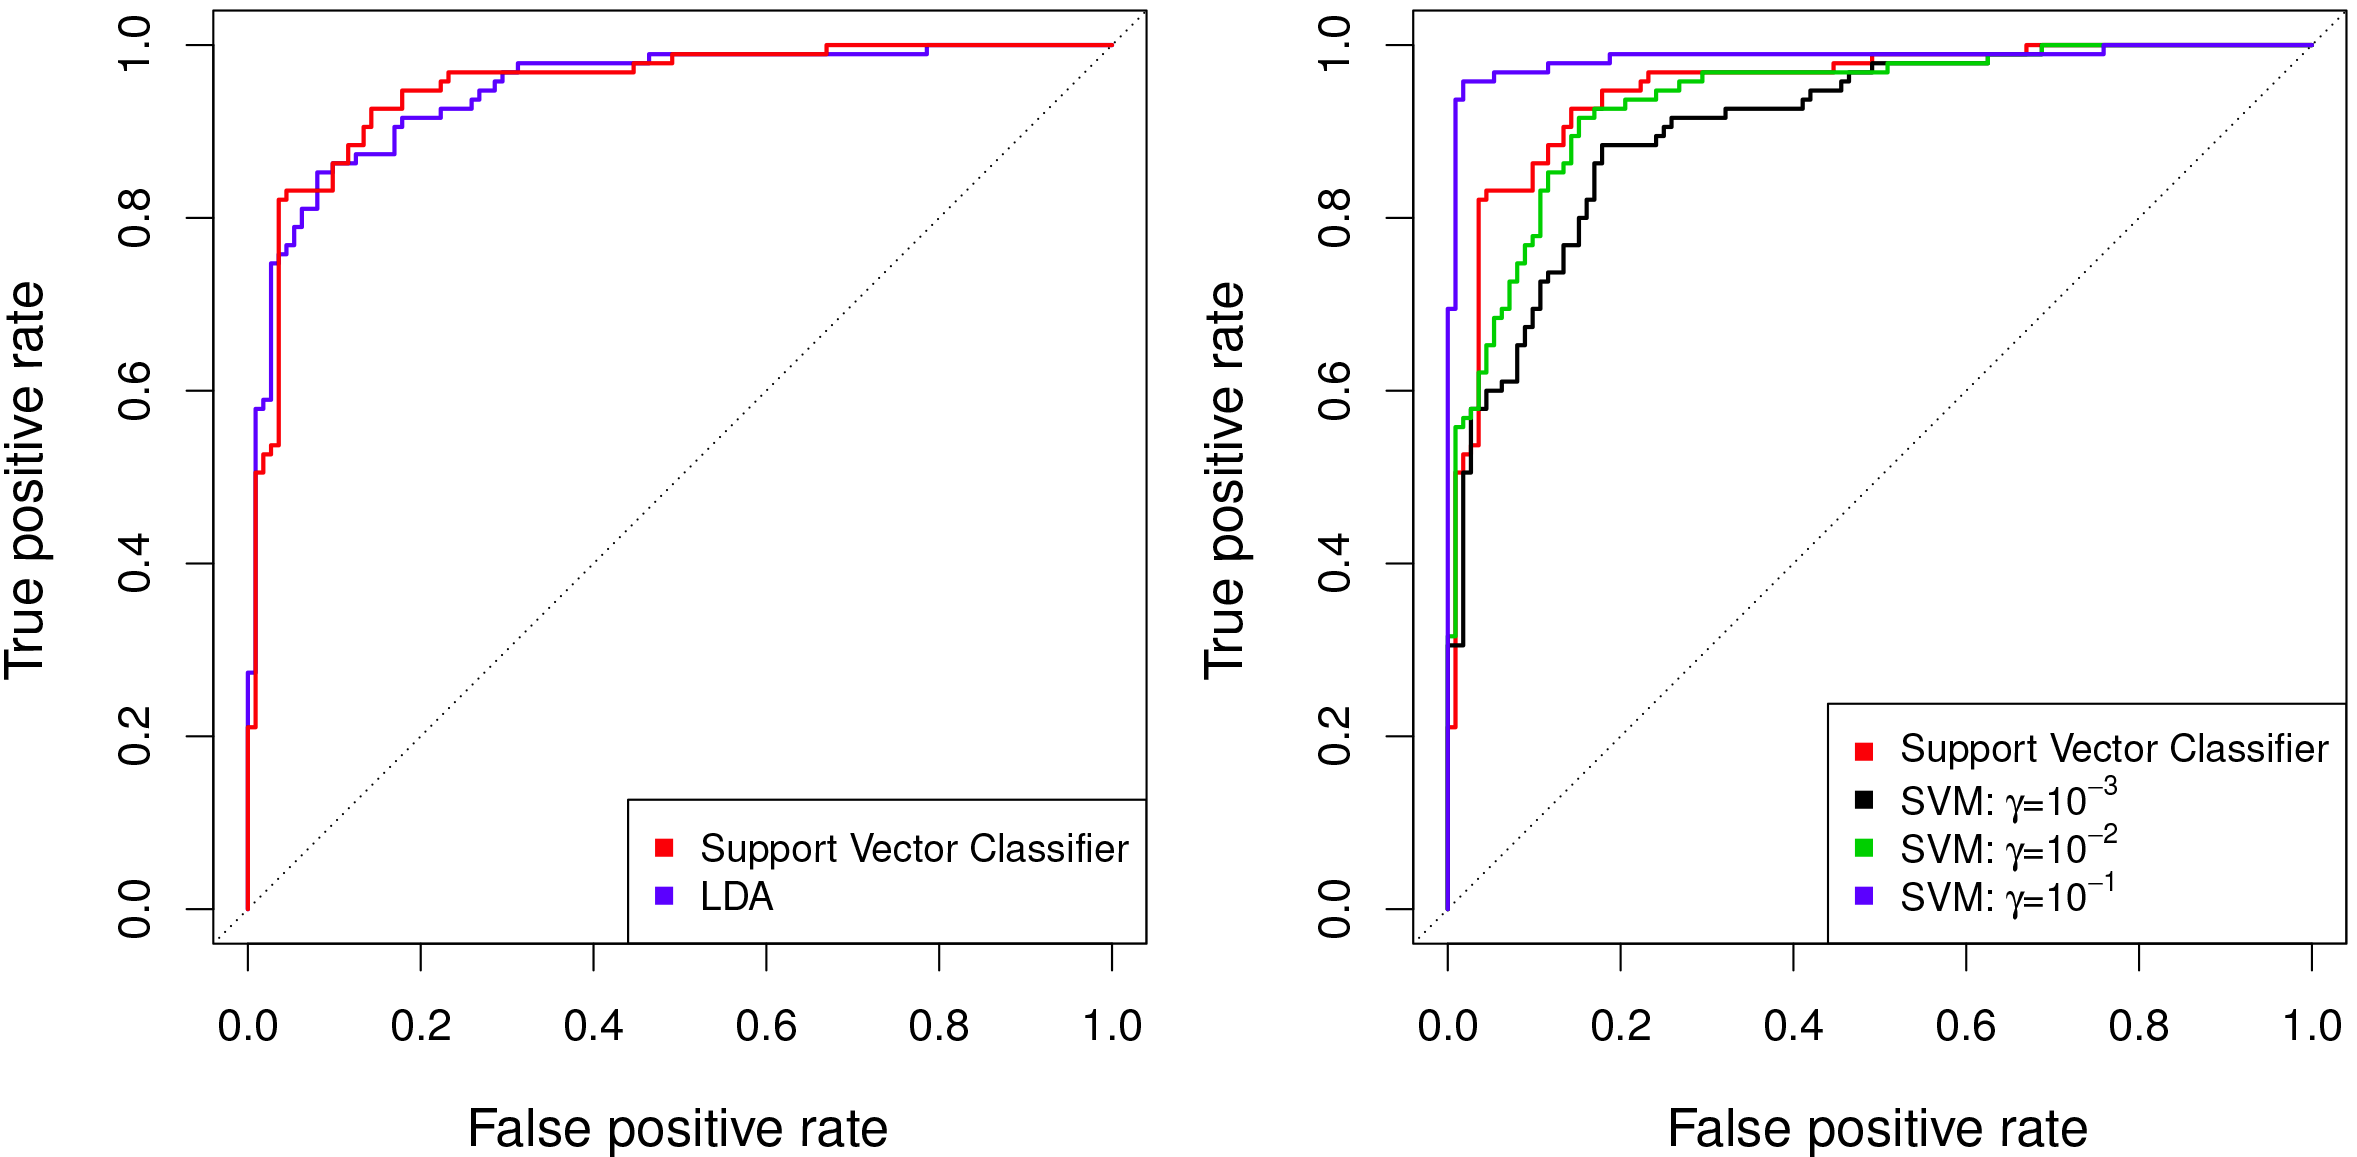
\includegraphics{../ISLR/Chapter9/9.10.png}
\caption{ISLR Figure 9.10}
\end{figure}

\begin{center}\rule{0.5\linewidth}{\linethickness}\end{center}

Heart data - test error.

\begin{figure}
\centering
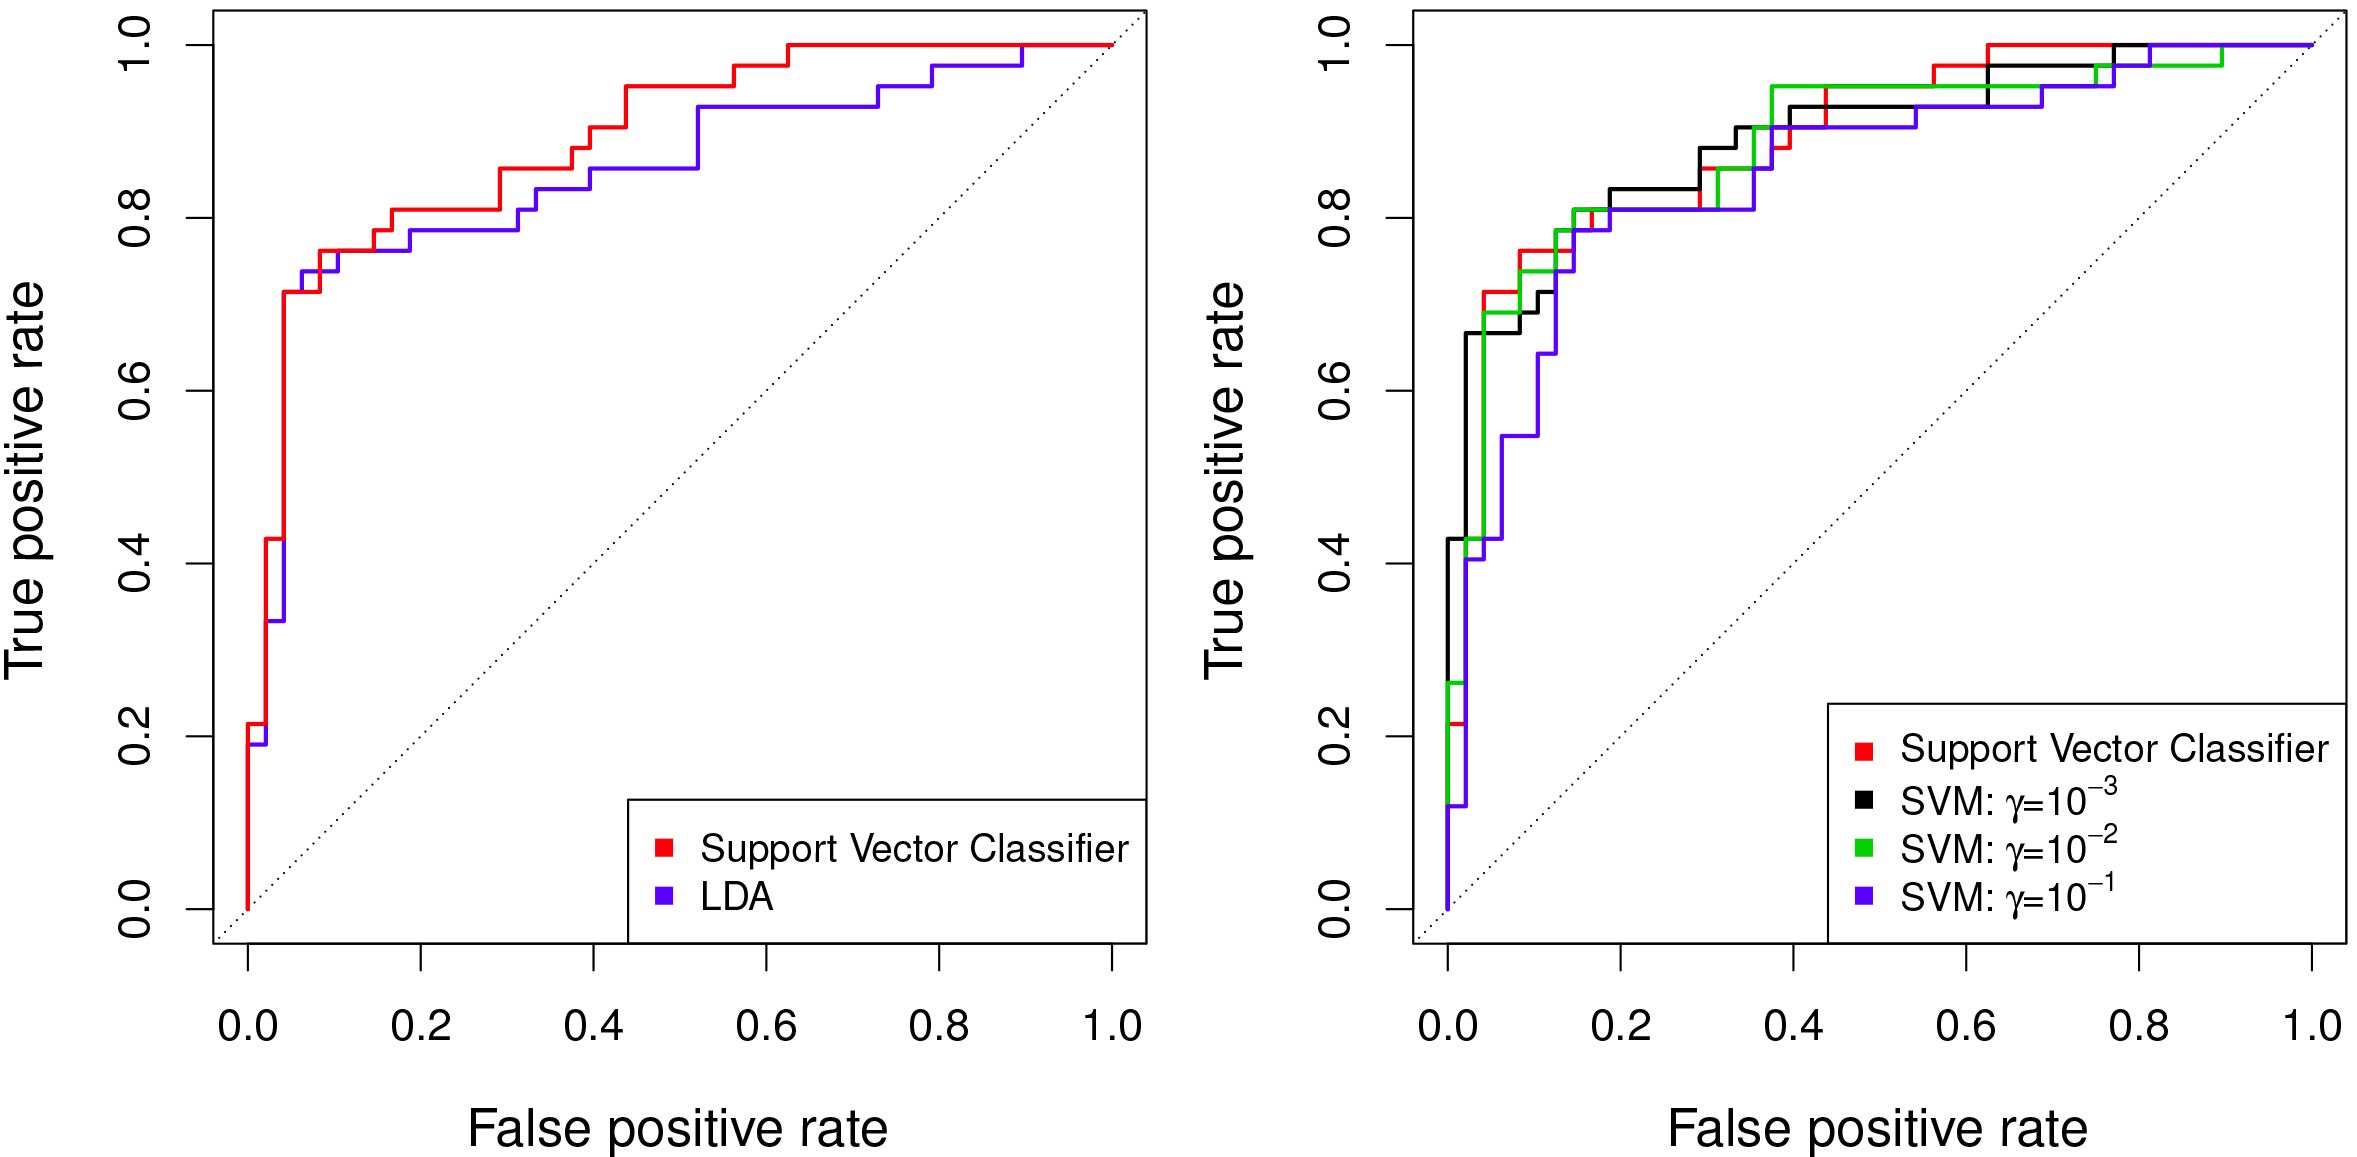
\includegraphics{../ISLR/Chapter9/9.11.png}
\caption{ISLR Figure 9.11}
\end{figure}

\begin{center}\rule{0.5\linewidth}{\linethickness}\end{center}

\hypertarget{example-forest-3}{%
\subsection{Example: forest 3}\label{example-forest-3}}

To illustrate the SVM we use the third training dataset (forest3) and
the third test set (seeds3). We use the \texttt{svm} function as before.
However, we now set
\texttt{kernel=\textquotesingle{}radial\textquotesingle{}} as we want a
non-linear decision boundary:

\begin{center}\rule{0.5\linewidth}{\linethickness}\end{center}

\footnotesize

\begin{Shaded}
\begin{Highlighting}[]
\KeywordTok{library}\NormalTok{(e1071)}
\NormalTok{forest3 =}\StringTok{ }\KeywordTok{read.table}\NormalTok{(}\DataTypeTok{file =} \StringTok{"forest3.txt"}\NormalTok{)}
\NormalTok{seeds3 =}\StringTok{ }\KeywordTok{read.table}\NormalTok{(}\DataTypeTok{file =} \StringTok{"seeds3.txt"}\NormalTok{)}
\NormalTok{train3 =}\StringTok{ }\KeywordTok{data.frame}\NormalTok{(}\DataTypeTok{x =}\NormalTok{ forest3[, }\DecValTok{1}\OperatorTok{:}\DecValTok{2}\NormalTok{], }\DataTypeTok{y =} \KeywordTok{as.factor}\NormalTok{(forest3[, }\DecValTok{3}\NormalTok{]))}
\NormalTok{test3 =}\StringTok{ }\KeywordTok{data.frame}\NormalTok{(}\DataTypeTok{x =}\NormalTok{ seeds3[, }\DecValTok{1}\OperatorTok{:}\DecValTok{2}\NormalTok{], }\DataTypeTok{y =} \KeywordTok{as.factor}\NormalTok{(seeds3[, }\DecValTok{3}\NormalTok{]))}
\end{Highlighting}
\end{Shaded}

\begin{center}\rule{0.5\linewidth}{\linethickness}\end{center}

\begin{Shaded}
\begin{Highlighting}[]
\NormalTok{svmfit_kernel1 =}\StringTok{ }\KeywordTok{svm}\NormalTok{(y }\OperatorTok{~}\StringTok{ }\NormalTok{., }\DataTypeTok{data =}\NormalTok{ train3, }\DataTypeTok{kernel =} \StringTok{"radial"}\NormalTok{, }\DataTypeTok{gamma =} \DecValTok{1}\NormalTok{, }
    \DataTypeTok{cost =} \DecValTok{10}\NormalTok{, }\DataTypeTok{scale =} \OtherTok{FALSE}\NormalTok{)}
\KeywordTok{plot}\NormalTok{(svmfit_kernel1, train3, }\DataTypeTok{col =} \KeywordTok{c}\NormalTok{(}\StringTok{"lightcoral"}\NormalTok{, }\StringTok{"lightgreen"}\NormalTok{))}
\end{Highlighting}
\end{Shaded}

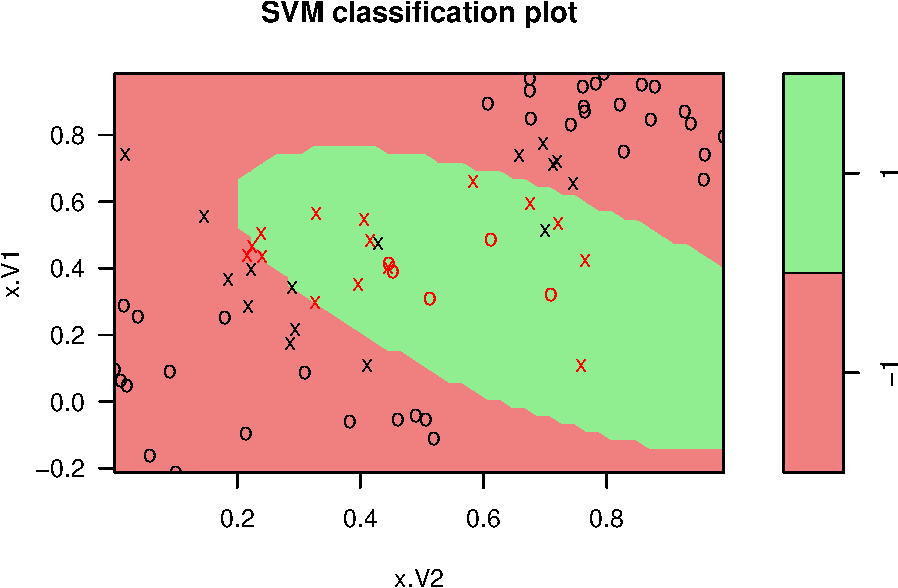
\includegraphics{9SVM_files/figure-latex/unnamed-chunk-21-1.pdf}

\begin{Shaded}
\begin{Highlighting}[]
\KeywordTok{summary}\NormalTok{(svmfit_kernel1)}
\end{Highlighting}
\end{Shaded}

\begin{verbatim}
## 
## Call:
## svm(formula = y ~ ., data = train3, kernel = "radial", gamma = 1, 
##     cost = 10, scale = FALSE)
## 
## 
## Parameters:
##    SVM-Type:  C-classification 
##  SVM-Kernel:  radial 
##        cost:  10 
## 
## Number of Support Vectors:  31
## 
##  ( 16 15 )
## 
## 
## Number of Classes:  2 
## 
## Levels: 
##  -1 1
\end{verbatim}

\normalsize

\begin{center}\rule{0.5\linewidth}{\linethickness}\end{center}

We could also try with a polynomial kernel with degree 4 as follows:

\footnotesize

\begin{Shaded}
\begin{Highlighting}[]
\NormalTok{svmfit_kernel2 =}\StringTok{ }\KeywordTok{svm}\NormalTok{(y }\OperatorTok{~}\StringTok{ }\NormalTok{., }\DataTypeTok{data =}\NormalTok{ train3, }\DataTypeTok{kernel =} \StringTok{"polynomial"}\NormalTok{, }\DataTypeTok{degree =} \DecValTok{4}\NormalTok{, }
    \DataTypeTok{cost =} \FloatTok{1e+05}\NormalTok{, }\DataTypeTok{scale =} \OtherTok{FALSE}\NormalTok{)}
\KeywordTok{plot}\NormalTok{(svmfit_kernel2, train3, }\DataTypeTok{col =} \KeywordTok{c}\NormalTok{(}\StringTok{"lightcoral"}\NormalTok{, }\StringTok{"lightgreen"}\NormalTok{))}
\end{Highlighting}
\end{Shaded}

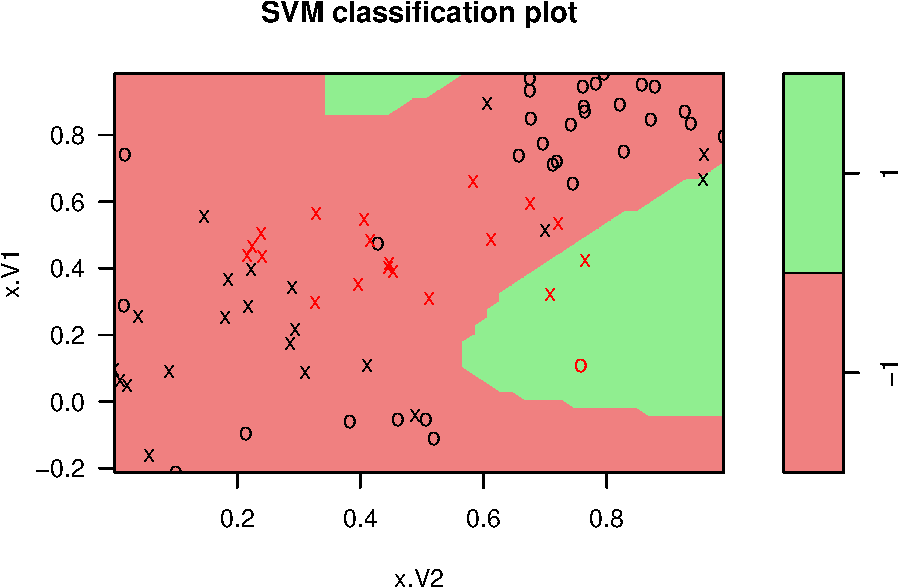
\includegraphics{9SVM_files/figure-latex/unnamed-chunk-22-1.pdf}

\begin{center}\rule{0.5\linewidth}{\linethickness}\end{center}

\begin{Shaded}
\begin{Highlighting}[]
\KeywordTok{summary}\NormalTok{(svmfit_kernel2)}
\end{Highlighting}
\end{Shaded}

\begin{verbatim}
## 
## Call:
## svm(formula = y ~ ., data = train3, kernel = "polynomial", degree = 4, 
##     cost = 1e+05, scale = FALSE)
## 
## 
## Parameters:
##    SVM-Type:  C-classification 
##  SVM-Kernel:  polynomial 
##        cost:  1e+05 
##      degree:  4 
##      coef.0:  0 
## 
## Number of Support Vectors:  40
## 
##  ( 21 19 )
## 
## 
## Number of Classes:  2 
## 
## Levels: 
##  -1 1
\end{verbatim}

\normalsize

\begin{center}\rule{0.5\linewidth}{\linethickness}\end{center}

For this dataset a radial kernel is a natural choice: A circular
decision boundary seems like a good idea. Thus, we proceed with
\texttt{kernel=\textquotesingle{}radial\textquotesingle{}}, and use the
\texttt{tune()} function to find the optimal tuning parameter \(C\):

\footnotesize

\begin{Shaded}
\begin{Highlighting}[]
\KeywordTok{set.seed}\NormalTok{(}\DecValTok{1}\NormalTok{)}
\NormalTok{CV_kernel =}\StringTok{ }\KeywordTok{tune}\NormalTok{(svm, y }\OperatorTok{~}\StringTok{ }\NormalTok{., }\DataTypeTok{data =}\NormalTok{ train3, }\DataTypeTok{kernel =} \StringTok{"radial"}\NormalTok{, }\DataTypeTok{gamma =} \DecValTok{1}\NormalTok{, }
    \DataTypeTok{ranges =} \KeywordTok{list}\NormalTok{(}\DataTypeTok{cost =} \KeywordTok{c}\NormalTok{(}\FloatTok{0.001}\NormalTok{, }\FloatTok{0.01}\NormalTok{, }\FloatTok{0.1}\NormalTok{, }\DecValTok{1}\NormalTok{, }\DecValTok{5}\NormalTok{, }\DecValTok{10}\NormalTok{, }\DecValTok{100}\NormalTok{)))}
\KeywordTok{summary}\NormalTok{(CV_kernel)}
\end{Highlighting}
\end{Shaded}

\begin{verbatim}
## 
## Parameter tuning of 'svm':
## 
## - sampling method: 10-fold cross validation 
## 
## - best parameters:
##  cost
##   100
## 
## - best performance: 0.1089286 
## 
## - Detailed performance results:
##    cost     error dispersion
## 1 1e-03 0.2732143  0.1472658
## 2 1e-02 0.2732143  0.1472658
## 3 1e-01 0.2732143  0.1472658
## 4 1e+00 0.1500000  0.1315463
## 5 5e+00 0.1357143  0.1226248
## 6 1e+01 0.1214286  0.1298110
## 7 1e+02 0.1089286  0.1066291
\end{verbatim}

\normalsize

\begin{center}\rule{0.5\linewidth}{\linethickness}\end{center}

The optimal \(C\) is 10. Next, we predict the class label of the seeds
in the test set with a model with C=10, make a confusion table and plot
the results:

\begin{Shaded}
\begin{Highlighting}[]
\NormalTok{bestmod_kernel =}\StringTok{ }\NormalTok{CV_kernel}\OperatorTok{$}\NormalTok{best.model}
\NormalTok{ypred_kernel =}\StringTok{ }\KeywordTok{predict}\NormalTok{(bestmod_kernel, test3)}
\end{Highlighting}
\end{Shaded}

\begin{center}\rule{0.5\linewidth}{\linethickness}\end{center}

\begin{Shaded}
\begin{Highlighting}[]
\KeywordTok{par}\NormalTok{(}\DataTypeTok{mfrow =} \KeywordTok{c}\NormalTok{(}\DecValTok{1}\NormalTok{, }\DecValTok{3}\NormalTok{))}
\KeywordTok{par}\NormalTok{(}\DataTypeTok{pty =} \StringTok{"s"}\NormalTok{)}
\KeywordTok{plot}\NormalTok{(}\OtherTok{NA}\NormalTok{, }\DataTypeTok{xlab =} \StringTok{"x1"}\NormalTok{, }\DataTypeTok{ylab =} \StringTok{"x2"}\NormalTok{, }\DataTypeTok{xlim =} \KeywordTok{c}\NormalTok{(}\DecValTok{0}\NormalTok{, }\DecValTok{1}\NormalTok{), }\DataTypeTok{ylim =} \KeywordTok{c}\NormalTok{(}\DecValTok{0}\NormalTok{, }\DecValTok{1}\NormalTok{))}
\KeywordTok{title}\NormalTok{(}\StringTok{"True class"}\NormalTok{)}
\KeywordTok{points}\NormalTok{(seeds3[seeds3[, }\DecValTok{3}\NormalTok{] }\OperatorTok{==}\StringTok{ }\DecValTok{-1}\NormalTok{, }\DecValTok{1}\OperatorTok{:}\DecValTok{2}\NormalTok{], }\DataTypeTok{pch =} \DecValTok{19}\NormalTok{, }\DataTypeTok{col =} \StringTok{"lightcoral"}\NormalTok{, }
    \DataTypeTok{cex =} \FloatTok{0.9}\NormalTok{)}
\KeywordTok{points}\NormalTok{(seeds3[seeds3[, }\DecValTok{3}\NormalTok{] }\OperatorTok{==}\StringTok{ }\DecValTok{1}\NormalTok{, }\DecValTok{1}\OperatorTok{:}\DecValTok{2}\NormalTok{], }\DataTypeTok{pch =} \DecValTok{19}\NormalTok{, }\DataTypeTok{col =} \StringTok{"darkseagreen"}\NormalTok{, }
    \DataTypeTok{cex =} \FloatTok{0.9}\NormalTok{)}
\KeywordTok{points}\NormalTok{(seeds3[}\KeywordTok{which}\NormalTok{(ypred_kernel }\OperatorTok{!=}\StringTok{ }\NormalTok{seeds3[, }\DecValTok{3}\NormalTok{]), }\DecValTok{1}\OperatorTok{:}\DecValTok{2}\NormalTok{], }\DataTypeTok{pch =} \DecValTok{21}\NormalTok{)  }\CommentTok{#Mark misclassification.}
\end{Highlighting}
\end{Shaded}

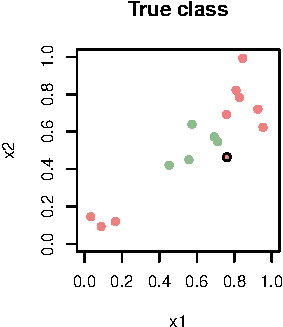
\includegraphics{9SVM_files/figure-latex/unnamed-chunk-26-1.pdf}

\begin{center}\rule{0.5\linewidth}{\linethickness}\end{center}

\begin{Shaded}
\begin{Highlighting}[]
\KeywordTok{plot}\NormalTok{(}\OtherTok{NA}\NormalTok{, }\DataTypeTok{xlab =} \StringTok{"x1"}\NormalTok{, }\DataTypeTok{ylab =} \StringTok{"x2"}\NormalTok{, }\DataTypeTok{xlim =} \KeywordTok{c}\NormalTok{(}\DecValTok{0}\NormalTok{, }\DecValTok{1}\NormalTok{), }\DataTypeTok{ylim =} \KeywordTok{c}\NormalTok{(}\DecValTok{0}\NormalTok{, }\DecValTok{1}\NormalTok{))}
\KeywordTok{title}\NormalTok{(}\StringTok{"Predicted class"}\NormalTok{)}
\KeywordTok{points}\NormalTok{(seeds3[ypred_kernel }\OperatorTok{==}\StringTok{ }\DecValTok{-1}\NormalTok{, }\DecValTok{1}\OperatorTok{:}\DecValTok{2}\NormalTok{], }\DataTypeTok{pch =} \DecValTok{19}\NormalTok{, }\DataTypeTok{col =} \StringTok{"lightcoral"}\NormalTok{, }
    \DataTypeTok{cex =} \FloatTok{0.9}\NormalTok{)}
\KeywordTok{points}\NormalTok{(seeds3[ypred_kernel }\OperatorTok{==}\StringTok{ }\DecValTok{1}\NormalTok{, }\DecValTok{1}\OperatorTok{:}\DecValTok{2}\NormalTok{], }\DataTypeTok{pch =} \DecValTok{19}\NormalTok{, }\DataTypeTok{col =} \StringTok{"darkseagreen"}\NormalTok{, }
    \DataTypeTok{cex =} \FloatTok{0.9}\NormalTok{)}
\KeywordTok{points}\NormalTok{(seeds3[}\KeywordTok{which}\NormalTok{(ypred_kernel }\OperatorTok{!=}\StringTok{ }\NormalTok{seeds3[, }\DecValTok{3}\NormalTok{]), }\DecValTok{1}\OperatorTok{:}\DecValTok{2}\NormalTok{], }\DataTypeTok{pch =} \DecValTok{21}\NormalTok{)  }\CommentTok{#Mark misclassification.}
\end{Highlighting}
\end{Shaded}

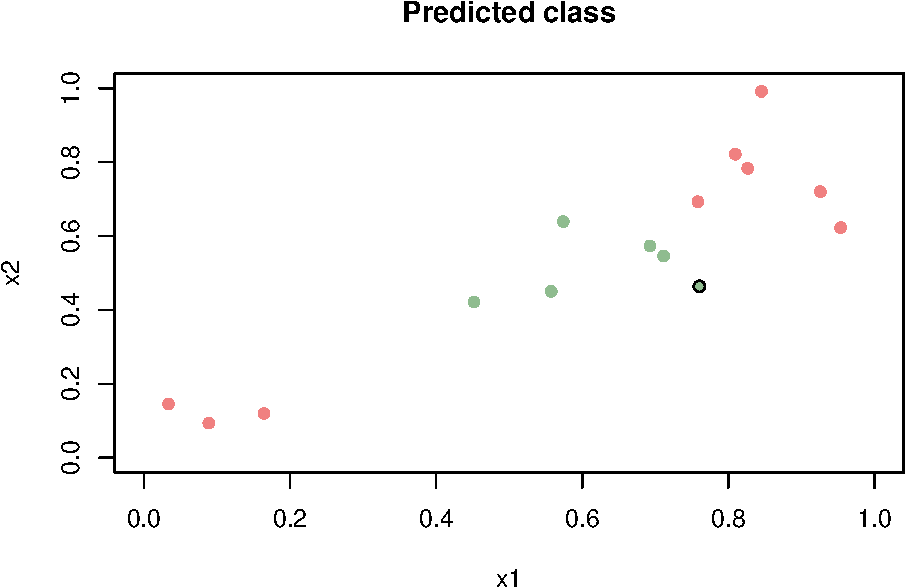
\includegraphics{9SVM_files/figure-latex/unnamed-chunk-27-1.pdf}

\begin{Shaded}
\begin{Highlighting}[]
\KeywordTok{table}\NormalTok{(}\DataTypeTok{predict =}\NormalTok{ ypred_kernel, }\DataTypeTok{truth =}\NormalTok{ test3[, }\DecValTok{3}\NormalTok{])}
\end{Highlighting}
\end{Shaded}

\begin{verbatim}
##        truth
## predict -1 1
##      -1  9 0
##      1   1 5
\end{verbatim}

Only one seed is misclassified.

\begin{center}\rule{0.5\linewidth}{\linethickness}\end{center}

\hypertarget{extensions}{%
\section{Extensions}\label{extensions}}

\hypertarget{more-than-two-classes}{%
\subsection{More than two classes}\label{more-than-two-classes}}

What if we have \(k\) classes?

\begin{itemize}
\tightlist
\item
  OVA: one-versus-all. Fit \(k\) different two-class SVMs
  \(f_k({\bf x})\) where one class is compared to all other classes.
  Classify a test observation to the class where \(f_k({\bf x}^*)\) is
  largest.
\item
  OVO: one-versus-one. \texttt{libsvm} uses this approach, in which
  \(k(k-1)/2\) binary classifiers are trained; the appropriate class is
  found by a voting scheme (the class that wins the most pairwise
  competitions are chosen).
\end{itemize}

\begin{center}\rule{0.5\linewidth}{\linethickness}\end{center}

\hypertarget{comparisons}{%
\section{ Comparisons}\label{comparisons}}

Focus is comparing the support vector classifier and logistic regression

It is possible to write the optimization problem for the support vector
classifier as a ``loss''+``penalty'':

\[\text{minimize}_{\boldsymbol \beta} \left\{ \sum_{i=1}^n \max(0,1-y_i f({\bf x}_i))+ \lambda \sum_{j=1}^p \beta_j^2 \right\}\]

\begin{itemize}
\item
  the loss is called \emph{hinge loss} - observe the max and 0 to
  explain why only support vectors contribute
\item
  the penalty is a ridge penalty
\item
  large \(\lambda\) gives \(\beta\)s small and more violations=high
  bias, but low variance
\item
  small \(\lambda\) gives \(\beta\)s large and less violations=low bias,
  but high variance
\end{itemize}

\begin{center}\rule{0.5\linewidth}{\linethickness}\end{center}

\begin{figure}
\centering
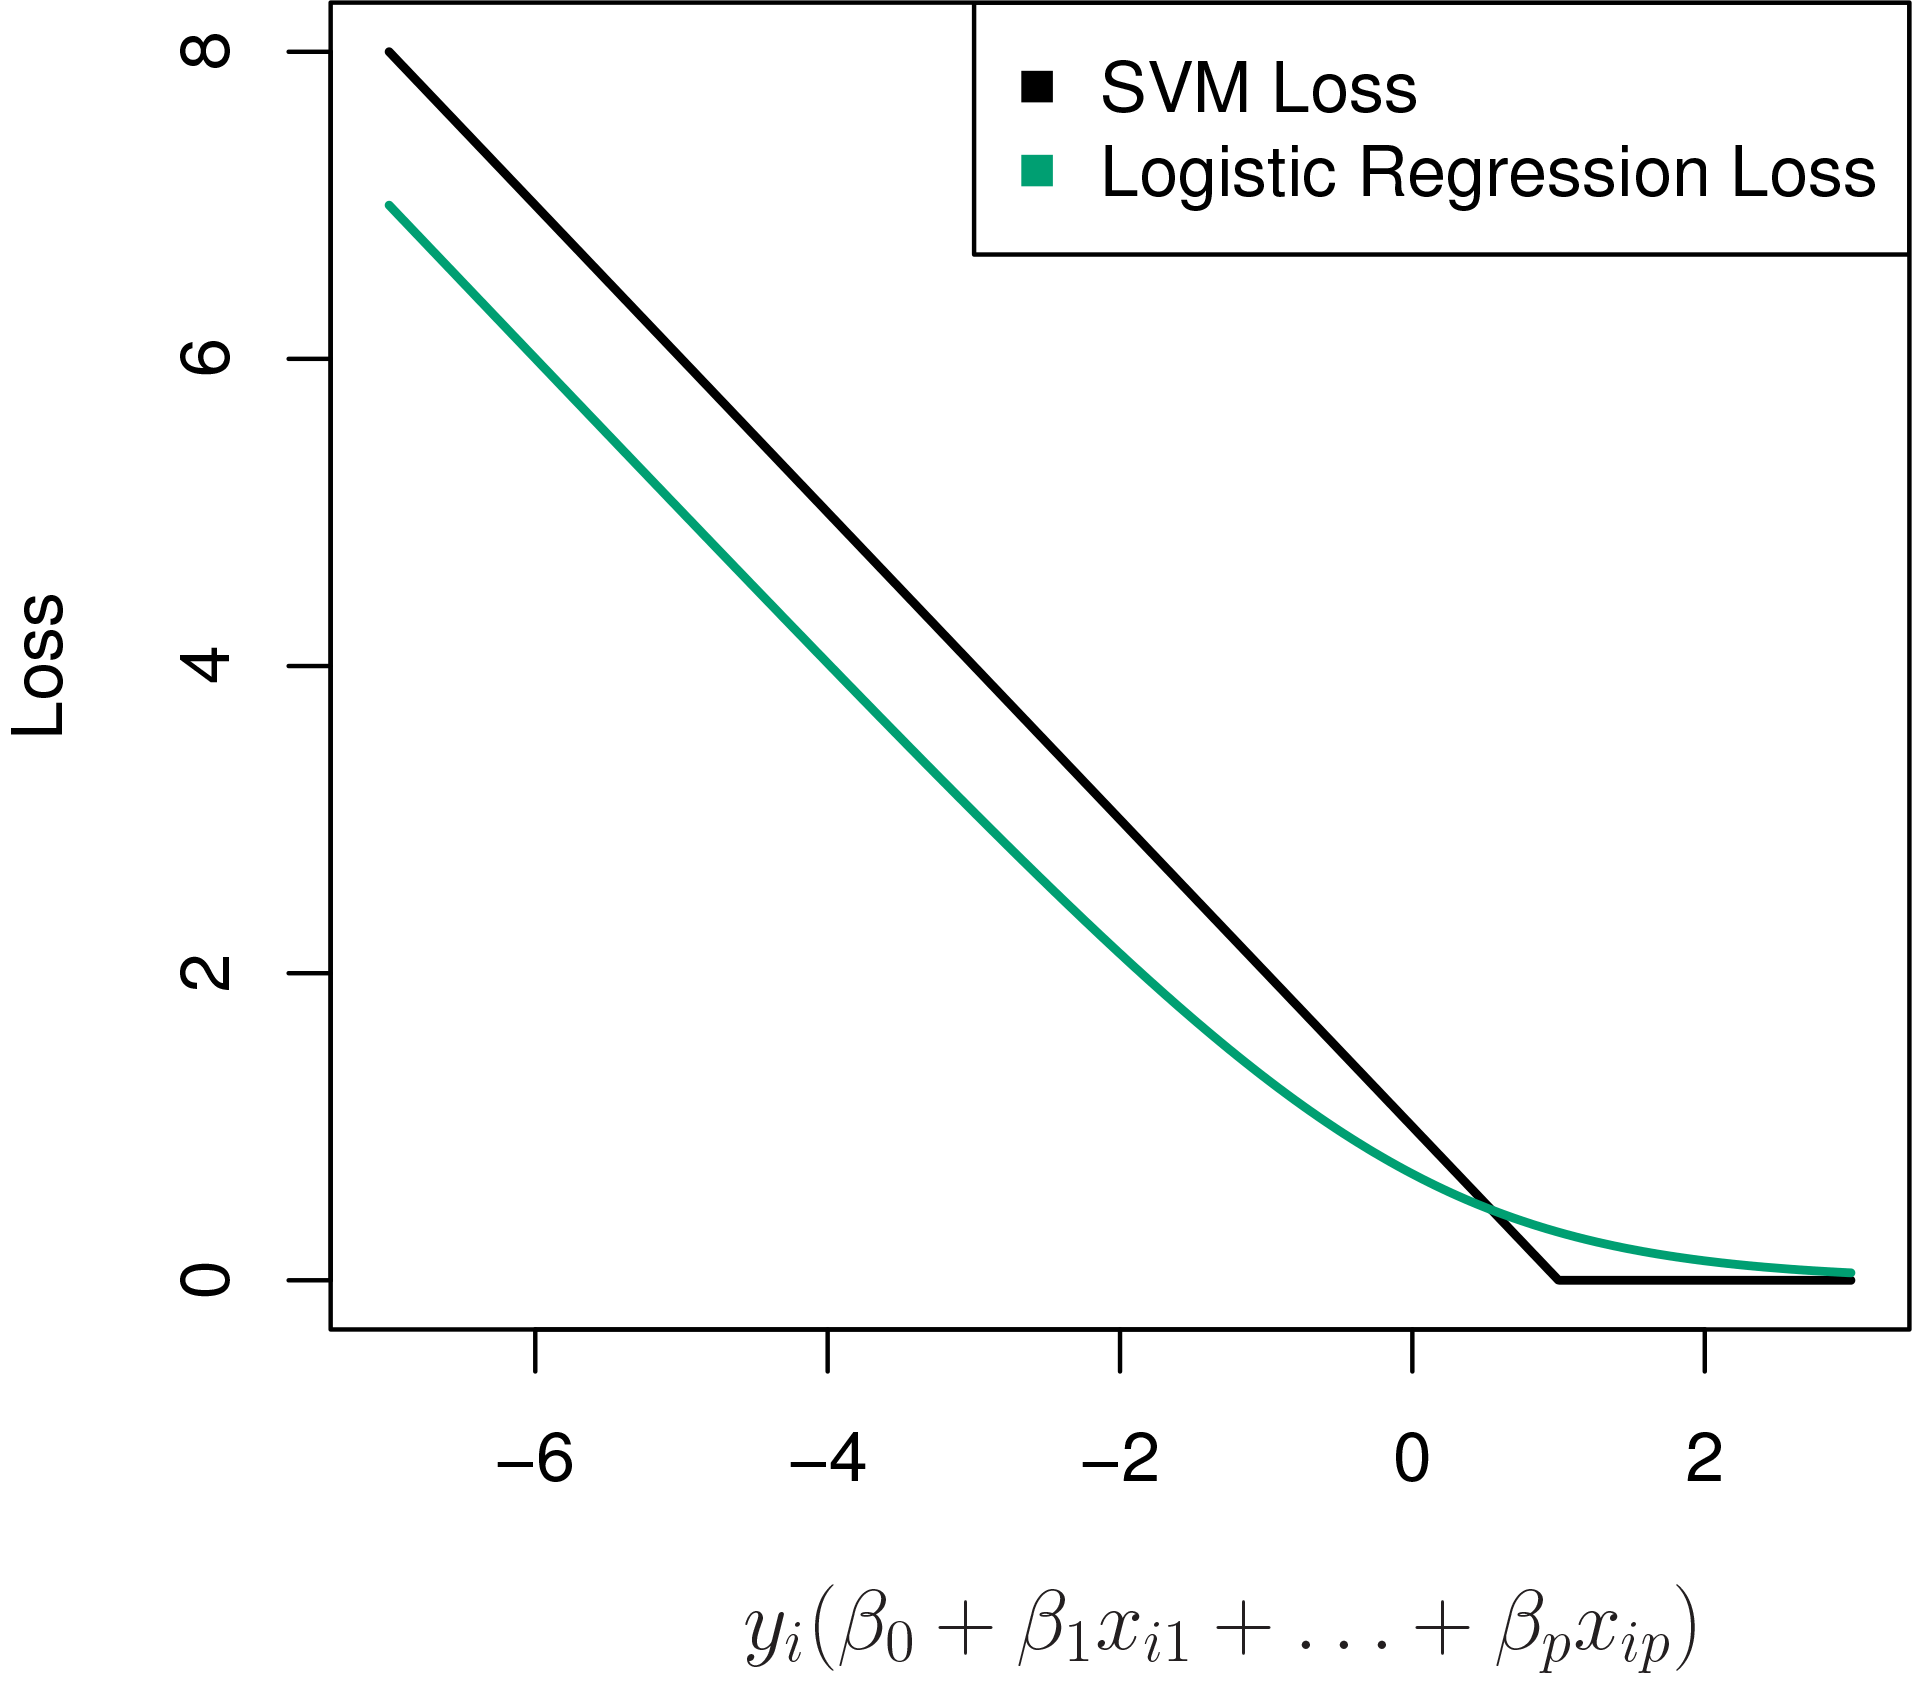
\includegraphics{../ISLR/Chapter9/9.12.png}
\caption{ISLR Figure 9.12: hinge loss - loss 0 for observations on the
correct side of the margin}
\end{figure}

\begin{center}\rule{0.5\linewidth}{\linethickness}\end{center}

\textbf{Hinge loss:} \[\max(0,1-y_if({\bf x}_i))\]

For comparison a logistic regression (with ridge penalty) would be
(binomial deviance with -1,1 coding of \(y\))

\[ \log(1+\exp(-y_i f({\bf x}_i)))\]

It can be shown that in logistic regression all observations contribute
weighted by \(p_i(1-p_i)\) (where \(p_i\) is probability for class 1),
that fade smoothly with distance to the decision boundary

It is possible to extend the logistic regression to include non-linear
terms, and ridge penalty.

\begin{center}\rule{0.5\linewidth}{\linethickness}\end{center}

\hypertarget{when-to-use-svm}{%
\subsection{When to use SVM?}\label{when-to-use-svm}}

\begin{itemize}
\tightlist
\item
  If classes are nearly separable SVM will perform better than logistic
  regression. (LDA will also perform better than logistic regression.)
\item
  and if not, then a ridge penalty version of logistic regression are
  very similar to SVM, and logistic regression will also give you
  probabilities for each class.
\item
  If class boundaries are non-linear then SVM is more popular, but
  kernel versions of logistic regression is possible, but more
  computationally expensive.
\end{itemize}

\begin{center}\rule{0.5\linewidth}{\linethickness}\end{center}

\hypertarget{summing-up}{%
\section{ Summing up }\label{summing-up}}

\begin{center}\rule{0.5\linewidth}{\linethickness}\end{center}

\begin{itemize}
\tightlist
\item
  We use methods from computer science, not probability models - but
  looks for a separating hyperplane in (an extended) feature space in
  the classification setting.
\item
  SVM is a widely successful and a ``must have tool''
\item
  Interpretation of SVM: all features are included and maybe not so easy
  to interpret (remember ridge-type penalty does not shrink to zero).
\item
  The budget must be chosen wisely, and a bad choice can lead to
  overfitting.
\item
  Not so easy to get class probabilites from SVM (what is done is
  actually to fit a logistic regression after fitting SVM).
\end{itemize}

\begin{center}\rule{0.5\linewidth}{\linethickness}\end{center}

\hypertarget{recommended-exercises}{%
\section{Recommended exercises}\label{recommended-exercises}}

\hypertarget{understanding-the-algorithms}{%
\subsection{1. Understanding the
algorithms:}\label{understanding-the-algorithms}}

\begin{itemize}
\tightlist
\item
  Exercise 1, 2 and 3 in the book.
\end{itemize}

\hypertarget{data-analysis}{%
\subsection{2. Data analysis}\label{data-analysis}}

\begin{itemize}
\item
  Go back and read in the \texttt{forest1} data (is located in the same
  place as \texttt{forest2}) and run the \texttt{svm} with a very high
  value for \texttt{cost}. The \texttt{forest1} is a separable problem.
\item
  Linear version of SVM: Making nicer plots for SVM from
  \href{https://www.youtube.com/watch?v=qhyyufR0930\&list=PL5-da3qGB5IDl6MkmovVdZwyYOhpCxo5o\&index=5}{Lab
  video}. Go through the code and see what is happening (and see the
  video if you want more explanation).
\end{itemize}

\begin{Shaded}
\begin{Highlighting}[]
\CommentTok{# code taken from video by Trevor Hastie linked above}
\KeywordTok{library}\NormalTok{(e1071)}
\CommentTok{# fake data}
\KeywordTok{set.seed}\NormalTok{(}\DecValTok{10111}\NormalTok{)}
\NormalTok{x =}\StringTok{ }\KeywordTok{matrix}\NormalTok{(}\KeywordTok{rnorm}\NormalTok{(}\DecValTok{40}\NormalTok{), }\DecValTok{20}\NormalTok{, }\DecValTok{2}\NormalTok{)}
\NormalTok{y =}\StringTok{ }\KeywordTok{rep}\NormalTok{(}\KeywordTok{c}\NormalTok{(}\OperatorTok{-}\DecValTok{1}\NormalTok{, }\DecValTok{1}\NormalTok{), }\KeywordTok{c}\NormalTok{(}\DecValTok{10}\NormalTok{, }\DecValTok{10}\NormalTok{))}
\NormalTok{x[y }\OperatorTok{==}\StringTok{ }\DecValTok{1}\NormalTok{, ] =}\StringTok{ }\NormalTok{x[y }\OperatorTok{==}\StringTok{ }\DecValTok{1}\NormalTok{, ] }\OperatorTok{+}\StringTok{ }\DecValTok{1}
\KeywordTok{plot}\NormalTok{(x, }\DataTypeTok{col =}\NormalTok{ y }\OperatorTok{+}\StringTok{ }\DecValTok{3}\NormalTok{, }\DataTypeTok{pch =} \DecValTok{19}\NormalTok{)}
\end{Highlighting}
\end{Shaded}

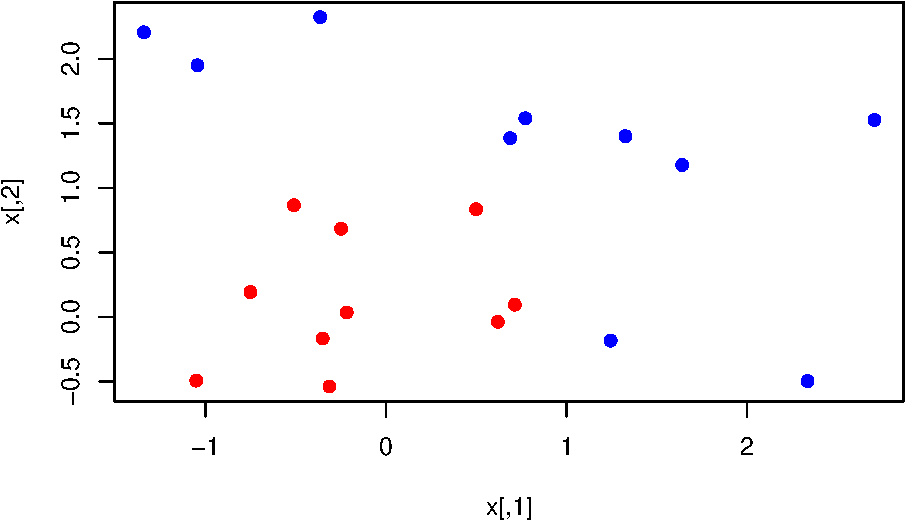
\includegraphics{9SVM_files/figure-latex/unnamed-chunk-28-1.pdf}

\begin{Shaded}
\begin{Highlighting}[]
\CommentTok{# calling svm}
\NormalTok{dat =}\StringTok{ }\KeywordTok{data.frame}\NormalTok{(x, }\DataTypeTok{y =} \KeywordTok{as.factor}\NormalTok{(y))}
\NormalTok{svmfit =}\StringTok{ }\KeywordTok{svm}\NormalTok{(y }\OperatorTok{~}\StringTok{ }\NormalTok{., }\DataTypeTok{data =}\NormalTok{ dat, }\DataTypeTok{kernel =} \StringTok{"linear"}\NormalTok{, }\DataTypeTok{cost =} \DecValTok{10}\NormalTok{, }\DataTypeTok{scale =} \OtherTok{FALSE}\NormalTok{)}
\KeywordTok{print}\NormalTok{(svmfit)}
\end{Highlighting}
\end{Shaded}

\begin{verbatim}
## 
## Call:
## svm(formula = y ~ ., data = dat, kernel = "linear", cost = 10, 
##     scale = FALSE)
## 
## 
## Parameters:
##    SVM-Type:  C-classification 
##  SVM-Kernel:  linear 
##        cost:  10 
## 
## Number of Support Vectors:  6
\end{verbatim}

\begin{Shaded}
\begin{Highlighting}[]
\CommentTok{# grid for plotting}
\NormalTok{make.grid =}\StringTok{ }\ControlFlowTok{function}\NormalTok{(x, }\DataTypeTok{n =} \DecValTok{75}\NormalTok{) \{}
\NormalTok{    grange =}\StringTok{ }\KeywordTok{apply}\NormalTok{(x, }\DecValTok{2}\NormalTok{, range)}
\NormalTok{    x1 =}\StringTok{ }\KeywordTok{seq}\NormalTok{(}\DataTypeTok{from =}\NormalTok{ grange[}\DecValTok{1}\NormalTok{, }\DecValTok{1}\NormalTok{], }\DataTypeTok{to =}\NormalTok{ grange[}\DecValTok{2}\NormalTok{, }\DecValTok{1}\NormalTok{], }\DataTypeTok{length =}\NormalTok{ n)}
\NormalTok{    x2 =}\StringTok{ }\KeywordTok{seq}\NormalTok{(}\DataTypeTok{from =}\NormalTok{ grange[}\DecValTok{1}\NormalTok{, }\DecValTok{2}\NormalTok{], }\DataTypeTok{to =}\NormalTok{ grange[}\DecValTok{2}\NormalTok{, }\DecValTok{2}\NormalTok{], }\DataTypeTok{length =}\NormalTok{ n)}
    \KeywordTok{expand.grid}\NormalTok{(}\DataTypeTok{X1 =}\NormalTok{ x1, }\DataTypeTok{X2 =}\NormalTok{ x2)}
\NormalTok{\}}
\NormalTok{xgrid =}\StringTok{ }\KeywordTok{make.grid}\NormalTok{(x)}
\NormalTok{ygrid =}\StringTok{ }\KeywordTok{predict}\NormalTok{(svmfit, xgrid)}
\KeywordTok{plot}\NormalTok{(xgrid, }\DataTypeTok{col =} \KeywordTok{c}\NormalTok{(}\StringTok{"red"}\NormalTok{, }\StringTok{"blue"}\NormalTok{)[}\KeywordTok{as.numeric}\NormalTok{(ygrid)], }\DataTypeTok{pch =} \DecValTok{20}\NormalTok{, }\DataTypeTok{cex =} \FloatTok{0.2}\NormalTok{)}
\KeywordTok{points}\NormalTok{(x, }\DataTypeTok{col =}\NormalTok{ y }\OperatorTok{+}\StringTok{ }\DecValTok{3}\NormalTok{, }\DataTypeTok{pch =} \DecValTok{19}\NormalTok{)}
\KeywordTok{points}\NormalTok{(x[svmfit}\OperatorTok{$}\NormalTok{index, ], }\DataTypeTok{pch =} \DecValTok{5}\NormalTok{, }\DataTypeTok{cex =} \DecValTok{2}\NormalTok{)}
\end{Highlighting}
\end{Shaded}

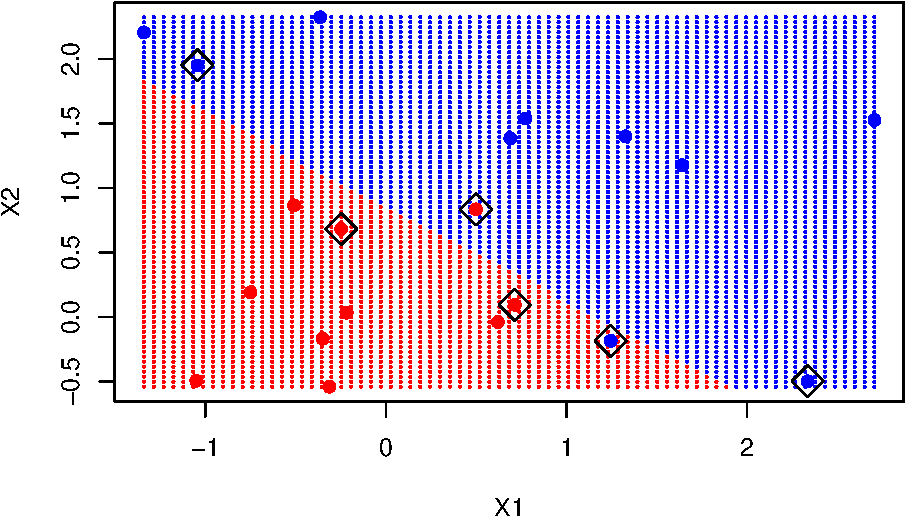
\includegraphics{9SVM_files/figure-latex/unnamed-chunk-28-2.pdf}

\begin{Shaded}
\begin{Highlighting}[]
\CommentTok{# more info on results - class boundary}

\NormalTok{beta =}\StringTok{ }\KeywordTok{drop}\NormalTok{(}\KeywordTok{t}\NormalTok{(svmfit}\OperatorTok{$}\NormalTok{coefs) }\OperatorTok\StringTok{ }\NormalTok{x[svmfit}\OperatorTok{$}\NormalTok{index, ])}
\NormalTok{beta0 =}\StringTok{ }\NormalTok{svmfit}\OperatorTok{$}\NormalTok{rho}
\KeywordTok{plot}\NormalTok{(xgrid, }\DataTypeTok{col =} \KeywordTok{c}\NormalTok{(}\StringTok{"red"}\NormalTok{, }\StringTok{"blue"}\NormalTok{)[}\KeywordTok{as.numeric}\NormalTok{(ygrid)], }\DataTypeTok{pch =} \DecValTok{20}\NormalTok{, }\DataTypeTok{cex =} \FloatTok{0.2}\NormalTok{)}
\KeywordTok{points}\NormalTok{(x, }\DataTypeTok{col =}\NormalTok{ y }\OperatorTok{+}\StringTok{ }\DecValTok{3}\NormalTok{, }\DataTypeTok{pch =} \DecValTok{19}\NormalTok{)}
\KeywordTok{points}\NormalTok{(x[svmfit}\OperatorTok{$}\NormalTok{index, ], }\DataTypeTok{pch =} \DecValTok{5}\NormalTok{, }\DataTypeTok{cex =} \DecValTok{2}\NormalTok{)}
\KeywordTok{abline}\NormalTok{(beta0}\OperatorTok{/}\NormalTok{beta[}\DecValTok{2}\NormalTok{], }\OperatorTok{-}\NormalTok{beta[}\DecValTok{1}\NormalTok{]}\OperatorTok{/}\NormalTok{beta[}\DecValTok{2}\NormalTok{])  }\CommentTok{#class boundary}
\KeywordTok{abline}\NormalTok{((beta0 }\OperatorTok{-}\StringTok{ }\DecValTok{1}\NormalTok{)}\OperatorTok{/}\NormalTok{beta[}\DecValTok{2}\NormalTok{], }\OperatorTok{-}\NormalTok{beta[}\DecValTok{1}\NormalTok{]}\OperatorTok{/}\NormalTok{beta[}\DecValTok{2}\NormalTok{])  }\CommentTok{#class boundary-margin}
\KeywordTok{abline}\NormalTok{((beta0 }\OperatorTok{+}\StringTok{ }\DecValTok{1}\NormalTok{)}\OperatorTok{/}\NormalTok{beta[}\DecValTok{2}\NormalTok{], }\OperatorTok{-}\NormalTok{beta[}\DecValTok{1}\NormalTok{]}\OperatorTok{/}\NormalTok{beta[}\DecValTok{2}\NormalTok{])  }\CommentTok{#class boundary+margin}
\end{Highlighting}
\end{Shaded}

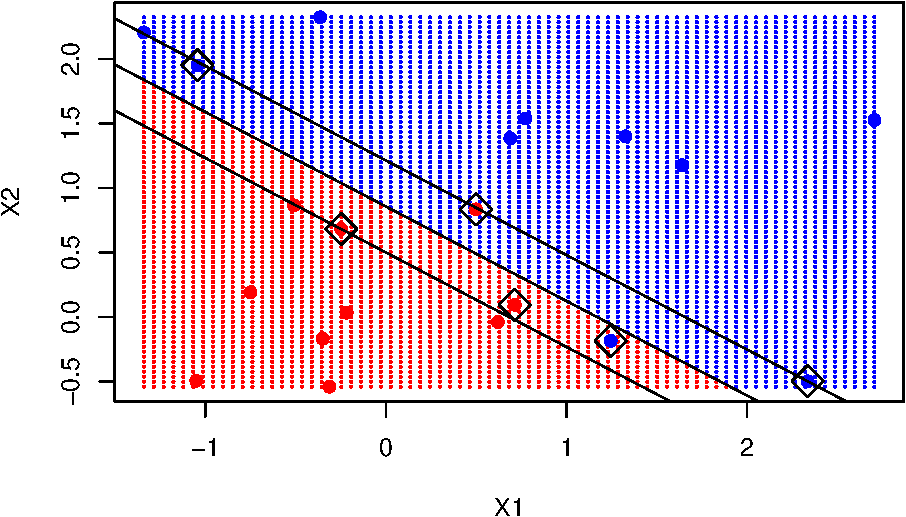
\includegraphics{9SVM_files/figure-latex/unnamed-chunk-28-3.pdf}

\begin{itemize}
\tightlist
\item
  SVM for non-linear class boundary using simulated data set from
  Friedman, Hastie, and Tibshirani (2001) where the truth is known
  (mixtures of normals probably).
\end{itemize}

\begin{Shaded}
\begin{Highlighting}[]
\KeywordTok{load}\NormalTok{(}\KeywordTok{url}\NormalTok{(}\StringTok{"https://web.stanford.edu/~hastie/ElemStatLearn/datasets/ESL.mixture.rda"}\NormalTok{))}
\KeywordTok{names}\NormalTok{(ESL.mixture)}
\end{Highlighting}
\end{Shaded}

\begin{verbatim}
## [1] "x"        "y"        "xnew"     "prob"     "marginal" "px1"     
## [7] "px2"      "means"
\end{verbatim}

\begin{Shaded}
\begin{Highlighting}[]
\KeywordTok{rm}\NormalTok{(x, y)}
\KeywordTok{attach}\NormalTok{(ESL.mixture)}

\KeywordTok{plot}\NormalTok{(x, }\DataTypeTok{col =}\NormalTok{ y }\OperatorTok{+}\StringTok{ }\DecValTok{1}\NormalTok{)}
\end{Highlighting}
\end{Shaded}

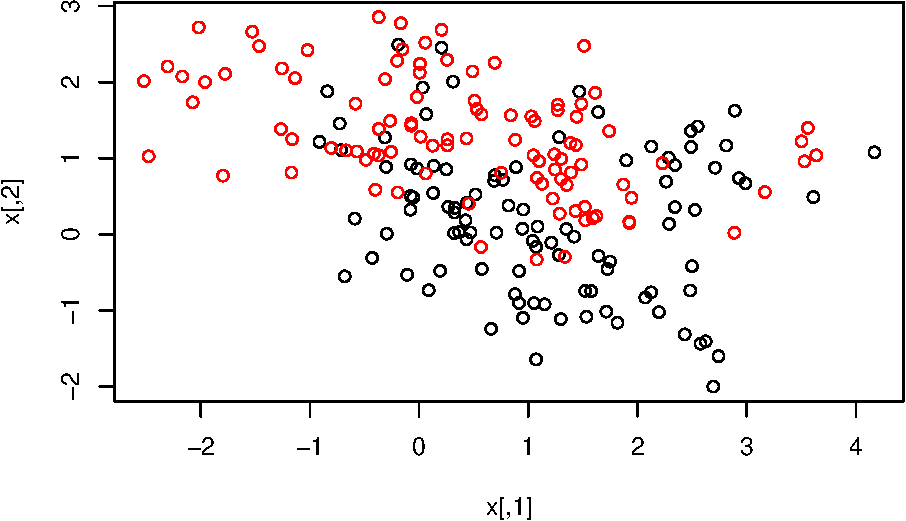
\includegraphics{9SVM_files/figure-latex/unnamed-chunk-29-1.pdf}

\begin{Shaded}
\begin{Highlighting}[]
\NormalTok{dat =}\StringTok{ }\KeywordTok{data.frame}\NormalTok{(}\DataTypeTok{y =} \KeywordTok{factor}\NormalTok{(y), x)}
\NormalTok{fit =}\StringTok{ }\KeywordTok{svm}\NormalTok{(}\KeywordTok{factor}\NormalTok{(y) }\OperatorTok{~}\StringTok{ }\NormalTok{., }\DataTypeTok{data =}\NormalTok{ dat, }\DataTypeTok{scale =} \OtherTok{FALSE}\NormalTok{, }\DataTypeTok{kernel =} \StringTok{"radial"}\NormalTok{, }
    \DataTypeTok{cost =} \DecValTok{5}\NormalTok{)}

\NormalTok{xgrid =}\StringTok{ }\KeywordTok{expand.grid}\NormalTok{(}\DataTypeTok{X1 =}\NormalTok{ px1, }\DataTypeTok{X2 =}\NormalTok{ px2)}
\NormalTok{ygrid =}\StringTok{ }\KeywordTok{predict}\NormalTok{(fit, xgrid)}
\KeywordTok{plot}\NormalTok{(xgrid, }\DataTypeTok{col =} \KeywordTok{as.numeric}\NormalTok{(ygrid), }\DataTypeTok{pch =} \DecValTok{20}\NormalTok{, }\DataTypeTok{cex =} \FloatTok{0.2}\NormalTok{)}
\KeywordTok{points}\NormalTok{(x, }\DataTypeTok{col =}\NormalTok{ y }\OperatorTok{+}\StringTok{ }\DecValTok{1}\NormalTok{, }\DataTypeTok{pch =} \DecValTok{19}\NormalTok{)}

\CommentTok{# decision boundary}
\NormalTok{func =}\StringTok{ }\KeywordTok{predict}\NormalTok{(fit, xgrid, }\DataTypeTok{decision.values =} \OtherTok{TRUE}\NormalTok{)}
\NormalTok{func =}\StringTok{ }\KeywordTok{attributes}\NormalTok{(func)}\OperatorTok{$}\NormalTok{decision}
\KeywordTok{contour}\NormalTok{(px1, px2, }\KeywordTok{matrix}\NormalTok{(func, }\DecValTok{69}\NormalTok{, }\DecValTok{99}\NormalTok{), }\DataTypeTok{level =} \DecValTok{0}\NormalTok{, }\DataTypeTok{add =} \OtherTok{TRUE}\NormalTok{)  }\CommentTok{#svm boundary}
\KeywordTok{contour}\NormalTok{(px1, px2, }\KeywordTok{matrix}\NormalTok{(prob, }\DecValTok{69}\NormalTok{, }\DecValTok{99}\NormalTok{), }\DataTypeTok{level =} \FloatTok{0.5}\NormalTok{, }\DataTypeTok{add =} \OtherTok{TRUE}\NormalTok{, }\DataTypeTok{col =} \StringTok{"blue"}\NormalTok{, }
    \DataTypeTok{lwd =} \DecValTok{2}\NormalTok{)  }\CommentTok{#truth}
\end{Highlighting}
\end{Shaded}

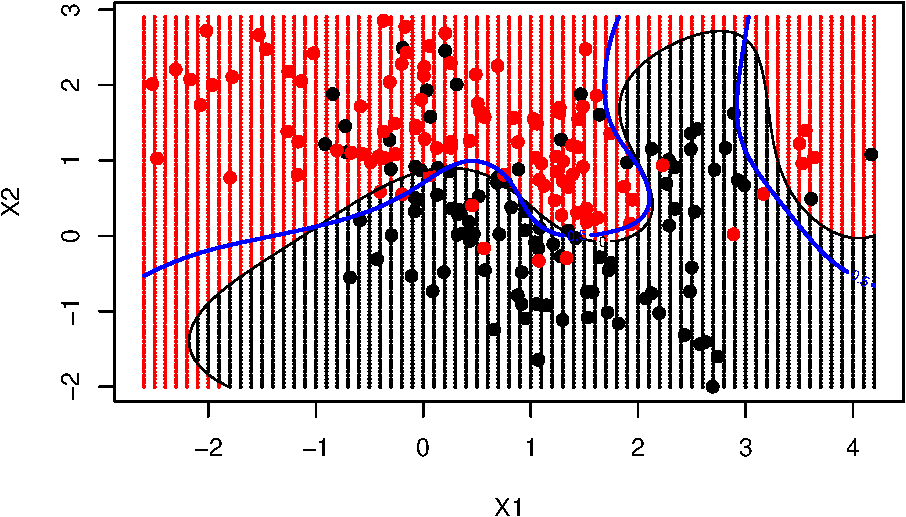
\includegraphics{9SVM_files/figure-latex/unnamed-chunk-29-2.pdf}

\hypertarget{compulsory-exercise-3-2018-problem-2---nonlinear-class-boundaries-and-support-vector-machine}{%
\subsection{Compulsory exercise 3 2018: Problem 2 - Nonlinear class
boundaries and support vector
machine}\label{compulsory-exercise-3-2018-problem-2---nonlinear-class-boundaries-and-support-vector-machine}}

\#\#3 a) Bayes decision boundary {[}1 point{]}

We will study classification applied to a simulated data set with two
classes from Friedman, Hastie, and Tibshirani (2001), where the data set
is supplied together with the Bayes decision boundary. The boundary is
plotted below, together with a training set.

\begin{Shaded}
\begin{Highlighting}[]
\KeywordTok{load}\NormalTok{(}\KeywordTok{url}\NormalTok{(}\StringTok{"https://web.stanford.edu/~hastie/ElemStatLearn/datasets/ESL.mixture.rda"}\NormalTok{))}
\CommentTok{# names(ESL.mixture) prob gives probabilites for each class when the}
\CommentTok{# true density functions are known px1 and px2 are coordinates in x1}
\CommentTok{# (length 69) and x2 (length 99) where class probabilites are}
\CommentTok{# calculated}
\KeywordTok{rm}\NormalTok{(x, y)}
\KeywordTok{attach}\NormalTok{(ESL.mixture)}
\NormalTok{dat =}\StringTok{ }\KeywordTok{data.frame}\NormalTok{(}\DataTypeTok{y =} \KeywordTok{factor}\NormalTok{(y), x)}
\NormalTok{xgrid =}\StringTok{ }\KeywordTok{expand.grid}\NormalTok{(}\DataTypeTok{X1 =}\NormalTok{ px1, }\DataTypeTok{X2 =}\NormalTok{ px2)}
\KeywordTok{par}\NormalTok{(}\DataTypeTok{pty =} \StringTok{"s"}\NormalTok{)}
\KeywordTok{plot}\NormalTok{(xgrid, }\DataTypeTok{pch =} \DecValTok{20}\NormalTok{, }\DataTypeTok{cex =} \FloatTok{0.2}\NormalTok{)}
\KeywordTok{points}\NormalTok{(x, }\DataTypeTok{col =}\NormalTok{ y }\OperatorTok{+}\StringTok{ }\DecValTok{1}\NormalTok{, }\DataTypeTok{pch =} \DecValTok{20}\NormalTok{)}
\KeywordTok{contour}\NormalTok{(px1, px2, }\KeywordTok{matrix}\NormalTok{(prob, }\DecValTok{69}\NormalTok{, }\DecValTok{99}\NormalTok{), }\DataTypeTok{level =} \FloatTok{0.5}\NormalTok{, }\DataTypeTok{add =} \OtherTok{TRUE}\NormalTok{, }\DataTypeTok{col =} \StringTok{"blue"}\NormalTok{, }
    \DataTypeTok{lwd =} \DecValTok{2}\NormalTok{)  }\CommentTok{#optimal boundary}
\end{Highlighting}
\end{Shaded}

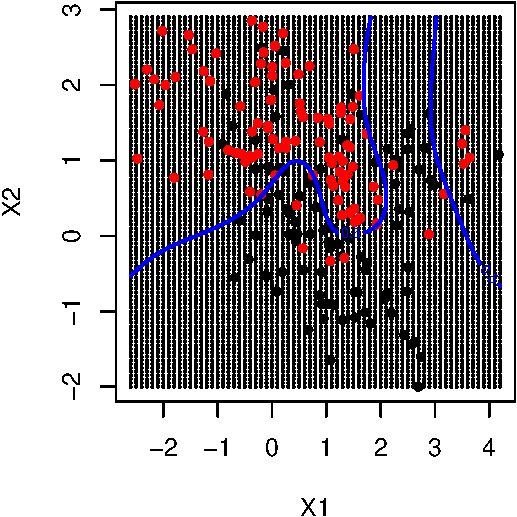
\includegraphics{9SVM_files/figure-latex/unnamed-chunk-30-1.pdf}

\begin{itemize}
\tightlist
\item
  Q11. What is a Bayes classifier, Bayes decision boundary and Bayes
  error rate? Hint: pages 37-39 in James et al. (2013).
\item
  Q12. When the Bayes decision boundary is known, do we then need a test
  set?
\end{itemize}

\hypertarget{b-support-vector-machine-1-point}{%
\subsubsection{b) Support vector machine {[}1
point{]}}\label{b-support-vector-machine-1-point}}

\begin{Shaded}
\begin{Highlighting}[]
\KeywordTok{library}\NormalTok{(e1071)}
\CommentTok{# support vector classifier}
\NormalTok{svcfits =}\StringTok{ }\KeywordTok{tune}\NormalTok{(svm, }\KeywordTok{factor}\NormalTok{(y) }\OperatorTok{~}\StringTok{ }\NormalTok{., }\DataTypeTok{data =}\NormalTok{ dat, }\DataTypeTok{scale =} \OtherTok{FALSE}\NormalTok{, }\DataTypeTok{kernel =} \StringTok{"linear"}\NormalTok{, }
    \DataTypeTok{ranges =} \KeywordTok{list}\NormalTok{(}\DataTypeTok{cost =} \KeywordTok{c}\NormalTok{(}\FloatTok{0.01}\NormalTok{, }\FloatTok{0.1}\NormalTok{, }\DecValTok{1}\NormalTok{, }\DecValTok{5}\NormalTok{, }\DecValTok{10}\NormalTok{)))}
\KeywordTok{summary}\NormalTok{(svcfits)}
\end{Highlighting}
\end{Shaded}

\begin{verbatim}
## 
## Parameter tuning of 'svm':
## 
## - sampling method: 10-fold cross validation 
## 
## - best parameters:
##  cost
##  0.01
## 
## - best performance: 0.27 
## 
## - Detailed performance results:
##    cost error dispersion
## 1  0.01 0.270 0.11595018
## 2  0.10 0.290 0.07745967
## 3  1.00 0.295 0.07619420
## 4  5.00 0.295 0.07619420
## 5 10.00 0.300 0.07817360
\end{verbatim}

\begin{Shaded}
\begin{Highlighting}[]
\NormalTok{svcfit =}\StringTok{ }\KeywordTok{svm}\NormalTok{(}\KeywordTok{factor}\NormalTok{(y) }\OperatorTok{~}\StringTok{ }\NormalTok{., }\DataTypeTok{data =}\NormalTok{ dat, }\DataTypeTok{scale =} \OtherTok{FALSE}\NormalTok{, }\DataTypeTok{kernel =} \StringTok{"linear"}\NormalTok{, }
    \DataTypeTok{cost =} \FloatTok{0.01}\NormalTok{)}
\CommentTok{# support vector machine with radial kernel}
\KeywordTok{set.seed}\NormalTok{(}\DecValTok{4268}\NormalTok{)}
\NormalTok{svmfits =}\StringTok{ }\KeywordTok{tune}\NormalTok{(svm, }\KeywordTok{factor}\NormalTok{(y) }\OperatorTok{~}\StringTok{ }\NormalTok{., }\DataTypeTok{data =}\NormalTok{ dat, }\DataTypeTok{scale =} \OtherTok{FALSE}\NormalTok{, }\DataTypeTok{kernel =} \StringTok{"radial"}\NormalTok{, }
    \DataTypeTok{ranges =} \KeywordTok{list}\NormalTok{(}\DataTypeTok{cost =} \KeywordTok{c}\NormalTok{(}\FloatTok{0.01}\NormalTok{, }\FloatTok{0.1}\NormalTok{, }\DecValTok{1}\NormalTok{, }\DecValTok{5}\NormalTok{, }\DecValTok{10}\NormalTok{), }\DataTypeTok{gamma =} \KeywordTok{c}\NormalTok{(}\FloatTok{0.01}\NormalTok{, }\DecValTok{1}\NormalTok{, }\DecValTok{5}\NormalTok{, }
        \DecValTok{10}\NormalTok{)))}
\KeywordTok{summary}\NormalTok{(svmfits)}
\end{Highlighting}
\end{Shaded}

\begin{verbatim}
## 
## Parameter tuning of 'svm':
## 
## - sampling method: 10-fold cross validation 
## 
## - best parameters:
##  cost gamma
##     1     5
## 
## - best performance: 0.16 
## 
## - Detailed performance results:
##     cost gamma error dispersion
## 1   0.01  0.01 0.550 0.11547005
## 2   0.10  0.01 0.530 0.12064641
## 3   1.00  0.01 0.275 0.09204468
## 4   5.00  0.01 0.275 0.06346478
## 5  10.00  0.01 0.290 0.08432740
## 6   0.01  1.00 0.535 0.14539219
## 7   0.10  1.00 0.230 0.08232726
## 8   1.00  1.00 0.175 0.06770032
## 9   5.00  1.00 0.175 0.06770032
## 10 10.00  1.00 0.180 0.08881942
## 11  0.01  5.00 0.505 0.20608790
## 12  0.10  5.00 0.400 0.18708287
## 13  1.00  5.00 0.160 0.07745967
## 14  5.00  5.00 0.215 0.09143911
## 15 10.00  5.00 0.195 0.09559754
## 16  0.01 10.00 0.515 0.18566697
## 17  0.10 10.00 0.505 0.18173546
## 18  1.00 10.00 0.190 0.07745967
## 19  5.00 10.00 0.235 0.12483322
## 20 10.00 10.00 0.255 0.13006409
\end{verbatim}

\begin{Shaded}
\begin{Highlighting}[]
\NormalTok{svmfit =}\StringTok{ }\KeywordTok{svm}\NormalTok{(}\KeywordTok{factor}\NormalTok{(y) }\OperatorTok{~}\StringTok{ }\NormalTok{., }\DataTypeTok{data =}\NormalTok{ dat, }\DataTypeTok{scale =} \OtherTok{FALSE}\NormalTok{, }\DataTypeTok{kernel =} \StringTok{"radial"}\NormalTok{, }
    \DataTypeTok{cost =} \DecValTok{1}\NormalTok{, }\DataTypeTok{gamma =} \DecValTok{5}\NormalTok{)}

\CommentTok{# the same as in a - the Bayes boundary}
\KeywordTok{par}\NormalTok{(}\DataTypeTok{pty =} \StringTok{"s"}\NormalTok{)}
\KeywordTok{plot}\NormalTok{(xgrid, }\DataTypeTok{pch =} \DecValTok{20}\NormalTok{, }\DataTypeTok{cex =} \FloatTok{0.2}\NormalTok{)}
\KeywordTok{points}\NormalTok{(x, }\DataTypeTok{col =}\NormalTok{ y }\OperatorTok{+}\StringTok{ }\DecValTok{1}\NormalTok{, }\DataTypeTok{pch =} \DecValTok{20}\NormalTok{)}
\KeywordTok{contour}\NormalTok{(px1, px2, }\KeywordTok{matrix}\NormalTok{(prob, }\DecValTok{69}\NormalTok{, }\DecValTok{99}\NormalTok{), }\DataTypeTok{level =} \FloatTok{0.5}\NormalTok{, }\DataTypeTok{add =} \OtherTok{TRUE}\NormalTok{, }\DataTypeTok{col =} \StringTok{"blue"}\NormalTok{, }
    \DataTypeTok{lwd =} \DecValTok{2}\NormalTok{)  }\CommentTok{#optimal boundary}

\CommentTok{# decision boundaries from svc and svm added}
\NormalTok{svcfunc =}\StringTok{ }\KeywordTok{predict}\NormalTok{(svcfit, xgrid, }\DataTypeTok{decision.values =} \OtherTok{TRUE}\NormalTok{)}
\NormalTok{svcfunc =}\StringTok{ }\KeywordTok{attributes}\NormalTok{(svcfunc)}\OperatorTok{$}\NormalTok{decision}
\KeywordTok{contour}\NormalTok{(px1, px2, }\KeywordTok{matrix}\NormalTok{(svcfunc, }\DecValTok{69}\NormalTok{, }\DecValTok{99}\NormalTok{), }\DataTypeTok{level =} \DecValTok{0}\NormalTok{, }\DataTypeTok{add =} \OtherTok{TRUE}\NormalTok{, }\DataTypeTok{col =} \StringTok{"red"}\NormalTok{)  }\CommentTok{#svc boundary}
\NormalTok{svmfunc =}\StringTok{ }\KeywordTok{predict}\NormalTok{(svmfit, xgrid, }\DataTypeTok{decision.values =} \OtherTok{TRUE}\NormalTok{)}
\NormalTok{svmfunc =}\StringTok{ }\KeywordTok{attributes}\NormalTok{(svmfunc)}\OperatorTok{$}\NormalTok{decision}
\KeywordTok{contour}\NormalTok{(px1, px2, }\KeywordTok{matrix}\NormalTok{(svmfunc, }\DecValTok{69}\NormalTok{, }\DecValTok{99}\NormalTok{), }\DataTypeTok{level =} \DecValTok{0}\NormalTok{, }\DataTypeTok{add =} \OtherTok{TRUE}\NormalTok{, }\DataTypeTok{col =} \StringTok{"orange"}\NormalTok{)  }\CommentTok{#svm boundary}
\end{Highlighting}
\end{Shaded}

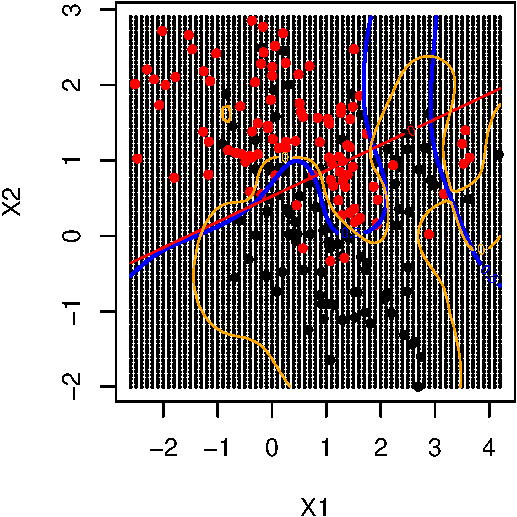
\includegraphics{9SVM_files/figure-latex/unnamed-chunk-31-1.pdf}

\begin{itemize}
\tightlist
\item
  Q13. What is the difference between a support vector classifier and a
  support vector machine?
\item
  Q14. What are parameters for the support vector classifier and the
  support vector machine? How are these chosen above?
\item
  Q15. How would you evaluate the support vector machine decision
  boundary compared to the Bayes decision boundary?
\end{itemize}

\begin{center}\rule{0.5\linewidth}{\linethickness}\end{center}

\hypertarget{r-packages}{%
\section{R packages}\label{r-packages}}

These packages needs to be install before knitting this R Markdown file.

\begin{Shaded}
\begin{Highlighting}[]
\KeywordTok{install.packages}\NormalTok{(e1071)}
\KeywordTok{install.packages}\NormalTok{(}\StringTok{"knitr"}\NormalTok{)}
\KeywordTok{install.packages}\NormalTok{(}\StringTok{"MASS"}\NormalTok{)}
\end{Highlighting}
\end{Shaded}

\begin{center}\rule{0.5\linewidth}{\linethickness}\end{center}

\hypertarget{references}{%
\section{References}\label{references}}

\begin{itemize}
\tightlist
\item
  \href{https://www.youtube.com/playlist?list=PL5-da3qGB5IDl6MkmovVdZwyYOhpCxo5o}{Videoes
  on YouTube by the authors of ISL, Chapter 9}, and corresponding
  \href{https://lagunita.stanford.edu/c4x/HumanitiesScience/StatLearning/asset/svm.pdf}{slides}
\item
  \href{https://rpubs.com/ppaquay/65566}{Solutions to exercises in the
  book, chapter 9}
\end{itemize}

\hypertarget{refs}{}
\leavevmode\hypertarget{ref-casi}{}%
Efron, Bradley, and Trevor Hastie. 2016. \emph{Computer Age Statistical
Inference - Algorithms, Evidence, and Data Science}. Cambridge
University Press.

\leavevmode\hypertarget{ref-ESL}{}%
Friedman, Jerome, Trevor Hastie, and Robert Tibshirani. 2001. \emph{The
Elements of Statistical Learning}. Vol. 1. Springer series in statistics
New York.

\leavevmode\hypertarget{ref-ISL}{}%
James, Gareth, Daniela Witten, Trevor Hastie, and Robert Tibshirani.
2013. \emph{An Introduction to Statistical Learning}. Vol. 112.
Springer.


\end{document}
